\documentclass[10pt]{report}

%% Text-Encoding festlegen. Mit utf8 oder utf8x funktionieren Umlaute wie gewohnt.
%% (mit Bibtex funktioniert nur utf8)
\usepackage[utf8x]{inputenc}

%% Sprachdatei für Trennregeln, Datum-Format und ähnliches festlegen
%\usepackage[german]{babel}  % nötig für Umlaute
\usepackage[ngerman, english]{babel}

%% optimiert das typographische Erscheinungsbild
\usepackage{microtype}

%% erlaubt Listen einfacher zu formatieren (bietet nosep für kompakte Listen)
\usepackage{enumitem}
%% erlaubt hübsche Tabellen über mehrere Seiten, beinhaltet booktabs (\toprule, \midrule, ...)
\usepackage{ctable}
%% ermöglicht farbigen Text ({\color{red} ...})
\usepackage{xcolor} 


\usepackage{mathrsfs}

%% erweiterte Funktionalität für Formeln (Pakete der American Mathematical Society)
\usepackage{amsfonts,amsmath,amsthm,amssymb}
 \numberwithin{equation}{chapter}

%% vordefinierte Einheiten, einfaches Angeben von Einheiten (\SI{8 \pm 1}{cm})
%%   die Unsicherheit soll mit +- abgetrennt werden
\usepackage[separate-uncertainty]{siunitx}
\sisetup{
    range-units = single,       % \SIrange soll die Einheit nur einmal anzeigen
    list-units  = repeat,       % \SIlist soll die Einheit wiederholen
}
%% bei siuntix funktioniert babel leider nicht
%% für englische Dokumente sollten diese Zeilen auskommentiert werden. 
\sisetup{
    range-phrase         = { bis },
    list-final-separator = { und },
%    list-pair-separator  = { und }, % an Uni noch nicht verfügbar
}

%% erlaubt es Bilddateien einzubinden
%% (ctable graphicx intern auch. Trotzdem ist es sinnvoll graphicx expilizt zu laden.
%%  Sonst entstehen schwehr verständliche Fehler, wenn ctable entfernt wird)
\usepackage{graphicx}
%% ermöglicht Bilder und Tabellen am eingegebenen Ort zu platzieren ([H])
\usepackage{float}
%% ermöglicht Unter-Bilder in einer figure-Umgebung
\usepackage{caption}
\captionsetup[figure]{font=footnotesize, labelfont=bf}
\captionsetup[subfigure]{labelformat=parens, labelsep=space, font=small}

\usepackage{subfig}
%% Grafik-Dateien werden in den folgenden Ordnern gesucht
\graphicspath{{img/}}
%% Grafikdateien haben die folgenden Endungen (höchste Priorität zu erst)
\DeclareGraphicsExtensions{.pdf,.png,.jpg}

%% Vertikaler Abstand zwischen Absätzen, Beginn eines Absatzes nicht einrücken
\usepackage{parskip}
% \setlength{\parskip}{0.6em}   % Vertikaler Abstand zwischen Absätzen anpassen 
% \setlength{\parindent}{0em}   % Einrück-Abstand anpassen 

%% zeige Labels im Seitenrand. Dies ist praktisch um Verweise zu kontrollieren
\usepackage[final]{showkeys} % die Option 'final' deaktiviert die Ausgabe von showkeys

\linespread{1.3}	% 1.3

%% Seiten-Layout einstellen
\usepackage[
 a4paper,
 total={13.8cm,21.7cm},          % Breite und Höhe des Inhalt-Bereichs
 top=40mm, left=36mm,        % Ränder oben und links
 headsep=10mm,               % Abstand des unteren Rands der Kopfzeile vom oberen Rand des Inhalts
 footskip=10mm               % Abstand des unteren des Inhalts zum oberen Rand der Fusszeile
% showframe					 % for troubleshooting
]{geometry}

%% Ermöglicht Links im PDF 
%%   sollte möglichst spät in der Präambel geladen werden
\usepackage[
 pdftex,                        % wir verwenden pdftex/pdflatex
 bookmarks=true,                % wir wollen auch im PDF-Reader ein Inhaltsverzeichnis
 bookmarksdepth=3,              % das Inhaltsverzeichnis soll 3 Tiefen enthalten
 colorlinks=true,               % Linktexte sollen Farbig sein 
 linkcolor=black,               % Links innerhalb des Dokuments bleiben schwarz
 citecolor=black,               % Links zu Quellenangaben bleiben ebenfalls schwarz
 urlcolor=black,                 % URL-Linktexte sollen blau dargestellt werden
%  pdfborder={0 0 0}              % Links im PDF erhalten keinen Rahmen, nur nötig wenn colorlinks=false
]{hyperref}

\usepackage{mathtools}

%% Angaben für die PDF-Eigenschaften
\hypersetup{
  pdfauthor = {Kevin Hauser},
  pdftitle = {KOMA Mitschrift},
  pdfsubject = {LaTeX},
  pdfkeywords = {LaTeX, Beispiel}
}



%% definiert \cref: Referenzen mit korrekter Bezeichnung (z.B. "Abbildung 1")
%%   die Nummer alleine ist weiter mittels \ref verfügbar
%% muss NACH 'hyperref' geladen werden
%\usepackage[german]{cleveref}
\usepackage[english, capitalise]{cleveref}


%================  for subfigure


%%%%%%%%%%%%%%%%%  additional libraries

% link: http://tex.stackexchange.com/questions/36524/how-to-put-a-framed-box-around-text-math-environment
\usepackage{mdframed}
\usepackage{lipsum} % for creating dummy text

\mdfdefinestyle{MyFrame}{%
    linecolor=black,
    outerlinewidth=2pt,
    roundcorner=20pt,
    innertopmargin=\baselineskip,
    innerbottommargin=\baselineskip,
%	leftmargin=1cm,
    innerrightmargin=20pt,
    innerleftmargin=20pt,
    backgroundcolor=gray!10!white,
    frametitlerule =true,
%    frametitlerulewidth=0.5pt,
	frametitlerulecolor=black
    }
    
    
\usepackage{physics}

\usepackage{siunitx}	% for typeset SI units correctly
    

%=======================================================================
% new commands
%=======================================================================

\newcommand{\myRef}[1]{
  Fig.\ref{#1}
}

\newcommand{\myEq}[1]{
  Eq.\ref{#1}
}

%\newcommand{\Tc}{
%  $T_c$
%}
%\newcommand{\lsco}[1][]{
%  LSCO#1
%}
%
\newcommand*{\NewPage}{
  \newpage\null\thispagestyle{empty}\newpage
}

\newcommand{\refEq}[1]{
  Eq  \ref{#1}
}

\newcommand{\OO}{ % typeset of large 'O' to indicate negleting higher orders (e.q. O(2))
  \mathcal{O}
}

\newcommand{\vc}[1]{ % typeset definition for vectors in math mode
  \mathbf{#1}
}
\DeclareMathOperator{\sign}{sign}





%=======================================================================
% TODO:
%=======================================================================
%   * find alternative for \underbrace{}. it does look ugly sometimes


% TODO: conecpts missing in script
%	* description of different quasi particles
%	* Kohn anomaly
%	* Peierls transition
%	* link of Kohn anomaly and Peierls transition to Lindhard potential
%	* Quantum oscillations 
%	* Onsager Relation


%========================================================================================================
%========================================================================================================
% Document
%========================================================================================================
%========================================================================================================

%% Angaben für \maketitle
\title{KOMA - Mitschrift}
\author{Kevin Hauser}
% \date{7. Mai 2013}             % ohne Angabe wird das heutig Datum verwendet

\begin{document}
\pagenumbering{roman} %
%=======================================================================
% Title page
%=======================================================================

\begin{titlepage}
    \begin{center}
%        \vspace*{1cm}
       
        \Huge
        \textbf{Mitschrift KOMA}
       
        \vspace{0.5cm}
        \Large

%        \includegraphics[width=0.4\textwidth]{{{img\manipulator.png}}}
 
 		\vspace{3.0cm}
		\begin{figure}[H]
 		\centering
 		
\includegraphics[width=0.5\textwidth]{{{../img/uzh_logo}}}
		\end{figure} 

       
        \vspace{1cm}
       
        %A thesis presented for the degree of\\
        %Doctor of Philosophy
       
       

       
       
        \vspace{1.5cm}
       
        Department of Physics\\
        University of Zurich\\
        \today
       
    \end{center}
\end{titlepage}


% empty page
\null
\thispagestyle{empty}
\setcounter{page}{2}


%=======================================================================
% Content
%=======================================================================


\begin{abstract}



\setcounter{page}{3}
\end{abstract}

\setcounter{page}{4}
\NewPage
\setcounter{page}{5}

\tableofcontents
\thispagestyle{empty} % don't show (roman) page number on titlepage


%=======================================================================
% Peierls Instability
%=======================================================================
%
% 19.09.2017


\chapter{Peierls Instability \& Charge Order}
\pagenumbering{arabic}

\section{Peierl Instability}


%=======================================================================
% Derivation of Kramers Kronig relation
%=======================================================================
%
% 25.09.2017

\chapter{Charge Order}

\section{From Causality to Kramer-Kronig relation}


Looking at a causal function $\tilde{\chi}(t)$, we can split it, like every analytical function, in an even $\chi_\text{even}(t)$ and an odd $\chi_\text{odd}(t)$ part.


\begin{minipage}{0.45\textwidth}
  \begin{equation*}
    \tilde{\chi}(t) ~~ = ~~ \left\{ \begin{array}{lc} 
      0        &  t < t_0 \\
      \chi(t)  &  t > t_0
    \end{array}\right.
  \end{equation*}
%   
\includegraphics[width=0.8\textwidth]{img/uzh_logo}
\end{minipage}
\begin{minipage}{0.1\textwidth}
\end{minipage}
\begin{minipage}{0.45\textwidth}
   
\includegraphics[width=0.8\textwidth]{../img/uzh_logo}
\end{minipage}

%Every function $\tilde{\chi}(t)$ can be divided in an even $\chi_{even}(t)$ and an odd $\chi_{odd}(t)$ part.

\begin{equation} \label{eq:even_odd}
\tilde{\chi}(t) ~~ = ~~ \frac{\tilde{\chi}(t) + \tilde{\chi}(-t)}{2} + \frac{\tilde{\chi}(t) - \tilde{\chi}(-t)}{2} ~~ = ~~ \chi_\text{even}(t) + \chi_\text{odd}(t)
\end{equation}


Multiplying the even part of this function with the signum function yields,

\begin{equation}
  \sign(t) \cdot \chi_\text{even} ~~ = ~~ \sign(t) \cdot \left\{ \frac{\tilde{\chi}(t)}{2} + \frac{\tilde{\chi}(-t)}{2} \right\} ~~ = ~~~\frac{\tilde{\chi}(t)}{2} - \frac{\tilde{\chi}(t)}{2} ~~ = ~~ \chi_\text{odd}(t)
\end{equation}


Using this relation to replace $\chi_\text{odd}(t)$ in \refEq{eq:even_odd}.


\begin{equation}
\tilde{\chi}(t) ~~ = ~~ \chi_\text{even} + \chi_\text{odd} ~~ = ~~ \underbrace{(1 + \sign(t))}_\text{step function} \cdot \chi_\text{even}(t) ~~ = ~~ \sigma(t) \cdot \chi_\text{even}(t)
\end{equation}


\begin{align}
  \chi_\text{odd}(\omega) ~~& =~~ \int \chi_\text{odd}(t) \cdot e^{i\omega t}\ dt
  ~~=~~ \int_{-\infty}^\infty \chi_\text{odd}(t) \cdot
  \{ \underbrace{\cos(\omega t)}_\text{even} + i\underbrace{\sin(\omega t)}_\text{odd} \}\ dt \nonumber \\
  ~~& =~~ i \int_{-\infty}^{\infty} \chi_\text{odd}(t) \cdot \sin(\omega t)\ dt ~~=~~ \chi''(\omega)
\end{align}


\subsubsection{Example: Damped Harmonic Oscillator}

The differential equation of a driven damped harmonic oscillation is given as

\begin{equation} \label{eq:damped_osc_DE}
  \Ddot{x}(t) ~+~ \gamma \dot{x}(t) ~+~ \omega_0^2 x(t) ~~=~~ f(t)
\end{equation}

where $\gamma$ is the damping coefficient and $\omega_0$ is the resonsance frequency.
The solution to this differential equation can be found rather easy by transforming it to the Fourier space.
%Transforming this equatin to Fourier space the solution function can be found rather easy

\begin{equation}
  -\omega^2 x(\omega) ~-~ i \omega \gamma x(\omega) ~+~ \omega_0^2 x(\omega) ~~=~~ f(\omega)
\end{equation}

%Our system can be characterised by defining the response function in Fourier space as
%We define the response function $\chi(t)$ and its Fourier transform

We define the systems response function in Fourier space as

\begin{equation} \label{eq:damped_osc_respond}
  \chi(\omega) ~~\equiv~~ \frac{x(\omega)}{f(\omega)} ~~=~~ \frac{1}{\omega_0^2 - \omega^2 + i\gamma\omega} ~~=~~ | \chi(\omega)| \{\cos(\phi) + i\sin(\phi) \}
\end{equation}

The benefit of doing so lays in the fact, that $\chi(\omega)$ depends solely on the system specific 	quantities like the resonance frequency $\omega_0$ and the damping coefficient $\gamma$.

In that sense the response function is characteristic to your system and doesn't depend on the applied driving force $f(\omega)$. This is handy because as soon as we have determined $\chi(\omega)$ for a given system, we can find the Fourier transform of the solution to \refEq{eq:damped_osc_DE} for various driving forces by just multipling the fourier transforms of the repsonse function and the driving force 

\begin{equation}
  x(\omega) ~~=~~ \chi(\omega) \cdot f(\omega) 
  ~~=~~ f(\omega) |\chi(\omega)| \{\cos(\phi(\omega)) +i \sin(\phi(\omega))\}
\end{equation}

on the left side we described the repsonse function in terms of its magnitude $|\chi(\omega)|$ and its frequency dependent phase $\phi(\omega)$.


%Because $\chi(\omega)$ is independent of the applied driving force $f(\omega)$, we have to calculate it only once for a given system. We are then able to determine the solution to \refEq{eg:damped_osc_DE} for different driving forces by just multiplying the Fourier transforms of the repsonse function and the driving force

Splitting the response function up in a real and imaginary part we get

\begin{align}
  \Re\ \chi(\omega) ~& \equiv~ \chi'(\omega) ~=~ \frac{\omega^2_0 - \omega}{(\omega^2-\omega^2_0)^2 + \omega^2 \gamma^2} \\
  \Im\ \chi(\omega) ~& \equiv~ \chi''(\omega) ~=~ \frac{\gamma \omega}{(\omega^2 - \omega^2_0)^2 + \omega^2 \gamma^2}
\end{align}

%The solution of this problem is then given in Fourier space as
%Wit the help of the response function we can give an expression for the 


To illustrate that this solution is correct, we look at the special case were the driving force is a harmonic oscillation

\begin{equation}
  f(t) ~=~ f_0 \cos(\omega_0 t) ~~~\Rightarrow~~~ f(\omega) 
  ~=~ f_0 \left( \delta(\omega_0 - \omega) + \delta(\omega_0 + \omega) \right)
\end{equation}


As an ansatz for a solution of \refEq{eq:damped_osc_DE} we choose

\begin{equation}
  x(t) ~~=~~ f_0 | \chi(\omega) | \cos(\omega t - \phi)
\end{equation}


We check if this ansatz is correct by calculating its Fourier transform

\begin{equation}
  x(\omega) ~~=~~ \int x(t)\ e^{i\omega t}\ dt 
  ~~=~~ f_0 |\chi(\omega)| \int \cos(\omega 1 - \phi)\ e^{i\omega t} dt 
  ~~=~~ f_0 | \chi(\omega) \int \left\{... \right\} 
\end{equation}

\textcolor{red}{equation not complete}


%=======================================================================
% Quantum Oscillations & ARPES - Techniques to measure Fermi surface
%=======================================================================
%
% 2.10.2017

\chapter{Quantum Oscillations \& ARPES}



%=======================================================================
% Quantum Oscillations / Onsager Relations
%=======================================================================
%
% 3.10.2017
\section{Quantum Oscillations}

\subsection{Onsager Relation}

\begin{equation}
  S \cdot \left( \frac{1}{B_{n+1}} ~-~ \frac{1}{B_n} \right) ~~=~~ \frac{2 \pi e}{\hbar}
\end{equation}

$S$ is the Fermi surface ($S=\pi k_F^2$.

\begin{equation}
  F ~~\equiv~~ \left( \frac{1}{B_{n+1}} ~-~ \frac{1}{B_n} \right)^{-1}
\end{equation}

\begin{equation}
  F ~~=~~ \frac{\Phi_0}{2 \pi^2} \cdot S
\end{equation}

where $\Phi_0 = \frac{h}{2e} = \text{Flux Quantum}$




%=======================================================================
% Scattering experiment
%=======================================================================
%
% 3.10.2017
\section{Angle Resolved Photoemission Spectroscopy}

\subsection{Scattering Experiment}

\textcolor{red}{sketch scattering experiment}

\subsection{Fermis Golder Rule}

\begin{equation}
  W ~~\propto~~ | \langle \vc{k}_f | V(\vc{r}) | \vc{k}_i \rangle |^2
\end{equation}


\subsection{Angle Resolved Photoemission spectroscopy}


\textcolor{red}{adapt ARPES section from BA}









%=======================================================================
% Phonons
%=======================================================================
%
% lec.notes 09.10.17 - first part

\chapter{Second Quantization}

\section{1D-Chain}

To have a fitst insight into second quantization, we look at a phonons emerging in a one dimensional chain of atoms

\textcolor{red}{skecht 1D lattice chain}


In the sketch above $u_i$ referes to the distance from equilibrium of the $i$-th atom, $p_i$ stands for the momentum of the $i$-th atom, $K$ is the spring constant and the lattice constant $a$.
The Hamiltonian of this system is given as

\begin{equation} \label{eq:ham_phonon_chain}
  H_\text{ph} ~~=~~ \sum_{j_1}^N \left\{ \frac{1}{2M} p_j^2 ~+~ \frac{1}{2} K (u_j - u_{j-1})^2 \right\}
\end{equation}

Since our problem has one dimension in real space it has also one dimension in the reciprocal space. We can introduce two length scales in the reciprocal space

\begin{enumerate}
  \item{The size of the one dim. unit cell defines the length of the reciprocal lattice vector $\vec{G}$ which is equal to the size of the Brillouin zone: $ G ~=~ 2\pi/a$}
  \item{The length $L$ of the chain of atoms in real space defines the lowest possible distance two points in reciprocal space can have $\Delta k_\text{min} ~=~ 2\pi/L$.}
\end{enumerate}


\textcolor{red}{sketch 1D k-space}


We now want to rewritte the Hamiltonian \refEq{eq:ham_phonon_chain} by replacing the distance from equilibrium and the momentum of the atoms by its fourer transformations

\begin{align}
  p_j ~=~ \frac{1}{\sqrt{N}} \sum_{k \in \text{BZ}} P_k e^{ikR^0_j} 
  ~~~~~~& \Longleftrightarrow~~~~~~
  P_k ~=~ \frac{1}{\sqrt{N}} \sum_{j} p_j e^{-ikR^0_j}\\
  u_j ~=~ \frac{1}{\sqrt{N}} \sum_{k \in \text{BZ}} U_k e^{ikR^0_j} 
  ~~~~~~& \Longleftrightarrow~~~~~~
  U_k ~=~ \frac{1}{\sqrt{N}} \sum_{j} u_j e^{-ikR^0_j}
\end{align}


Since it is a cumbersome procedure we look at the calculate the different terms from \refEq{eq:ham_phonon_chain} seperatly.
We start with $\sum_i p_j^2$:

\begin{equation}\label{eq:phonon_momentum}
  p_j ~~=~~ \frac{1}{\sqrt{N}} \sum_k P_k e^{ikR^0_j} ~~=~~ 
  \frac{1}{2\sqrt{N}} \bigg\{ 
  \underbrace{\sum_k P_k e^{ikR^0_j}}_\text{A} ~+~
  \underbrace{\sum_{-k} P_{-k} e^{-ikR^0_j}}_\text{B} \bigg\}
\end{equation}

The second equality sign holds because summing two times and sum and dividing by two gives the same result. Additionaly in the second sum we replaced $k \rightarrow -k$. No we can write

\begin{align}\label{eq:p_squared}
  p_j^2 ~~& =~~~\frac{1}{4N} \left( A^2 ~+~ B^2 ~+~ 2AB \right)
  ~~=~~ \frac{2}{4N} \sum_j AB \nonumber \\
  ~~& =~~ \frac{1}{2N} \sum_j \sum_k \sum_{-k} P_k P_{-k}
  ~~=~~ \sum_k P_k P_{-k}
\end{align}
\textcolor{red}{is this correct?}

To get to this result $\sum_j = e^{ikR^0_j} = \delta(k)$ was used.
For evaluating now $\sum_j (u_j - u_{j-1})^2$ we use

\begin{equation}
  u_j ~~=~~~\Bigg\{ \underbrace{\sum_k u_k e^{ikR_j^0}}_\text{A'} ~+~
  \underbrace{\sum_{-k} u_{-k} e^{-ikR_j^0}}_\text{B'} \Bigg\}
\end{equation}
\begin{align}
  u_{j-1} ~~& =~~ \frac{1}{\sqrt{N}} \sum_k u_k e^{ikR_j^0} e^{-ika}\nonumber \\
  ~~& =~~ \frac{1}{2\sqrt{N}} \Bigg\{ \sum_k u_k e^{ikR_j^0} e^{-ika} ~+~
  \sum_{-k} u_{-k} e^{-ikR_j^0} e^{ika} \Bigg\}
\end{align}

To get the final expression for $u_{j-1}$ we used $R_{j-1}^0=r_j^0-a$.

\begin{align}
  \sum_j (u_j ~-~ u_{j-i})^2 ~~& =~~ \sum_j (u_j^2 ~+~ u_{j-1}^2 ~+~ 2u_j u_{j-1})\nonumber \\
  ~~& =~~ \sum_k \left\{ u_k u_{-k} ~+~ u_k u_{-k} ~-~ 2u_k u_{-k} \frac{e^{-ika} ~+~ e^{ika}}{2} \right\}\nonumber \\ 
  ~~& =~~ \sum_k 2 u_k u_{-k} \left\{1 ~-~ \cos(ka) \right\}\nonumber \\
  ~~& =~~ \sum_k 2 u_k u_{-k} \sin^2(ka/2)
\end{align}

In the step were the summing over $j$ changed to a summing over $k$ the same arguments as for \refEq{eq:p_squared} were used. As we already know from the \textit{introduction to solid state phyiscs} class, we can assign the argument of the sum in the final expression as the square of the phonon dispersion relation $\omega(k)$

\begin{equation}\label{eq:dispersion_relation}
  \omega(k) ~~=~~ \omega_k ~~=~~  \sqrt{\frac{2K}{M}(1-\cos(ka)} ~~=~~ 
  \sqrt{\frac{4K}{M}} |\sin(ka/2)|
\end{equation}

Pluggin our solutions for $\sum_j p_j^2$ and $\sum_j (u_j-u_{j-1})^2$ into \refEq{eq:ham_phonon_chain} yields

\begin{equation}\label{eq:ham_phonon_chain2}
  H_\text{ph} ~~=~~ \sum_{j=1}^N \left\{ \frac{1}{2M} P_k P_{-k} ~+~ \frac{M \omega_k^2}{2} u_k u_{-k} \right\} 
\end{equation}

This expression similar to the Hamilatonian from the harmonic oscillator. We therefore define the latter operators $b_k$ and $b_k^\dag$

\begin{align}
  b_k ~~& =~~ \frac{1}{\sqrt{2}} \left( \frac{u_k}{l_k} ~+~ i \frac{p_k}{\hbar/l_k} \right)\\
  b_k^\dag ~~& =~~ \frac{1}{\sqrt{2}} \left( \frac{u_k}{l_k} ~-~ i\frac{p_k}{\hbar/l_k} \right)
\end{align}

and rewrite $H_\text{ph}$ as 

\begin{equation}
  H_\text{ph} ~~=~~ \sum_k \hbar \omega_k (b^\dag_k b_k ~+~ 1)
\end{equation}

This analogy between the Hamiltonian from the harmonic oscillations and \refEq{eq:ham_phonon_chain2} emphasises that we can describe the state if excited phonons in a solid as a combination of different modes similar to the different modes of oscillations of an excited harmonic oscillator. Further we can use the latter operators applied to the vacuum state to describe the excited states mathematically.

\textcolor{red}{picture single atom phonon dispersion relation}
\textcolor{red}{picture two atom basis phonon dispersion relation}
\textcolor{red}{...if going down in temperature peierl transition occurs -> kohn anomaly}

\textcolor{red}{why is neutron scattering good for probing accustic bands? - check lecture notes for explanation}

\textcolor{red}{...neutrons only probe lattice and neglect electronic structure}


This way of decribing the physical processes in terms of latter operators can be extended much more. It turns out that it is a very convenient way of describing physical problems and is used broadly in all fields in condensed matter physics. We refere to this notation as \textbf{Second quantization}. In the next sections we will learn how to apply this formalism more generally. 



%=======================================================================
% Second quantization
%=======================================================================
%
% lec.notes 10.10.17 - first part
% lec-notes 16.10.17 - second part

\section{Second quantization: Free electron gas} % 10.10.17 - first part

Hamiltonian of a free electron gas can be written as. 

\begin{equation}
  H ~~=~~ \sum_{k \sigma} \frac{(\hbar \hat{k})^2}{2m} c_{k \sigma}^\dag c_{k \sigma}
\end{equation}


The ground state at $T=0K$ is create by applying the electron-creation operators $c_{k_i \uparrow}$ of the $i-\text{th}$ electron $e_{i \uparrow}$ to the vacuum state $|0\rangle$ for every electron that is present in the electron gas. 

\begin{equation}
  | \text{FS} \rangle ~~=~~ c_{k_{N/2} \uparrow} c_{k_{N/2} \downarrow} ... c_{k_1 \uparrow} c_{k_1 \downarrow} | 0 \rangle ~~=~~   
\end{equation}

To get the total number of electrons $N$ the number operator $\hat{N} = \sum_{k \sigma} c_{k\sigma}^\dag c_{k\sigma}$ can be applied on the ground state to the ground state $| \text{FS} \rangle$

\begin{equation}\label{eq:number_operator}
  N ~~=~~ \langle \text{FS} | \hat{N} | \text{FS} \rangle 
    ~~=~~ \langle \text{FS} | \sum_{k\sigma} c_{k\sigma}^\dag c_{k\sigma} | \text{FS} \rangle
\end{equation} 


For the ground state at $T=0$ the 

Since we consider a free electron gas in its ground state at $T=0K$ the momentum values $k$ are limited to lay inside a sphere with radius $k_F$. Furthermore we have to take into account that in the system under consideration the orientation  of the spin $\sigma$ doesn't matter. Therefore we can replace the sum $\sum_\sigma$ by a factor two. 


\begin{align}
  N ~~& =~~ \sum_{\mathbf{k} \sigma} \langle \text{FS} | c_{k\sigma}^\dag c_{k\sigma} | \text{FS} \rangle ~~=~~ 2 \sum_{|\mathbf{k}|\ \leq k_F} \langle \text{FS} | \text{FS} \rangle
  ~~=~~ 2V \int \frac{d^3k}{(2\pi)^3} \theta(k_F - |\mathbf{k}|) \langle \text{FS} | \text{FS} \rangle \nonumber \\
  ~~& =~~ \frac{2V}{(2\pi)^3} \underset{|\mathbf{k}| \leq k_F}{\int} d^3k
\end{align}

Solving this integral in spherical coordinates gives

\begin{equation}
  N ~~=~~ \frac{2V}{(2\pi)^3} \int_0^{k_F} dk k^2 \int_{-1}^1 d\cos(\vartheta) \int_0^{2\pi} d\phi
  ~~=~~ \frac{1}{3} \frac{V}{\pi^2} k_F^3
\end{equation}

From that equation we can determine the electron density  $n$ for a  three dimensional free electron gas at zero Temperature 

\begin{equation}\label{eq:el_density}
  n = N/V = k_F^3/(3\pi^2)
\end{equation}


As another example of the usage of second quantization we want to determine now the ground state energy $E_0$ of the free electron gas

\begin{align}
  E_0 ~~& =~~ \langle \text{FS} | H | \text{FS} \rangle 
  ~~=~~ \sum_{\mathbf{k} \sigma} \frac{\hbar \mathbf{k})^2}{2m} \langle \text{FS} | c^\dag_{\mathbf{k} \sigma} c_{\mathbf{k} \sigma} | \text{FS} \rangle
  ~~=~~ \frac{\hbar^2}{2m} \sum_{\mathbf{k}\sigma} k^2 \theta(|\mathbf{k}| - k_F) \nonumber \\ 
  ~~& =~~ 2 \frac{4\pi V}{(2\pi)^3} \frac{\hbar^2}{2m} \int dk \theta(|\mathbf{k}| - k_F) k^4\nonumber \\
  ~~& =~~ \frac{4\pi V}{(2\pi)^3} \frac{\hbar}{m} \frac{k_F^5}{5} ~~=~~ \frac{3}{5} N E_F
\end{align}

To get to the final expression we used the electron density from \refEq{eq:el_density} and the Fermi Energy $E_F = (\hbar k_F)^2/(2m)$. 



\subsubsection{Electron-Electron Interaction term}

The electron-electron interaction term in a material is given as

\begin{equation}
  V_\text{el-el} ~~=~~ \frac{1}{2V} \sum_{\sigma_1, \sigma_2} \sum_{k_1, k_2, q} 
  V_q c^\dag_{k_1, \sigma_1} c^\dag_{k_2, \sigma_2} c_{k_1+q, \sigma_1}, c_{k_2-q, \sigma_2} 
\end{equation}


To understand this expression better we look first at one single interaction between two electrons with initial momentum and spin $k_1, \sigma_1$ and $k_2, \sigma_2$. The spin doesn't change. When colliding the exchanged momentum due to the interaction term $V_q$, were we assume $q \neq 0$. The electron momenta in the final state are related by $k_1 + q = k_2$.

\begin{figure}
  \centering
  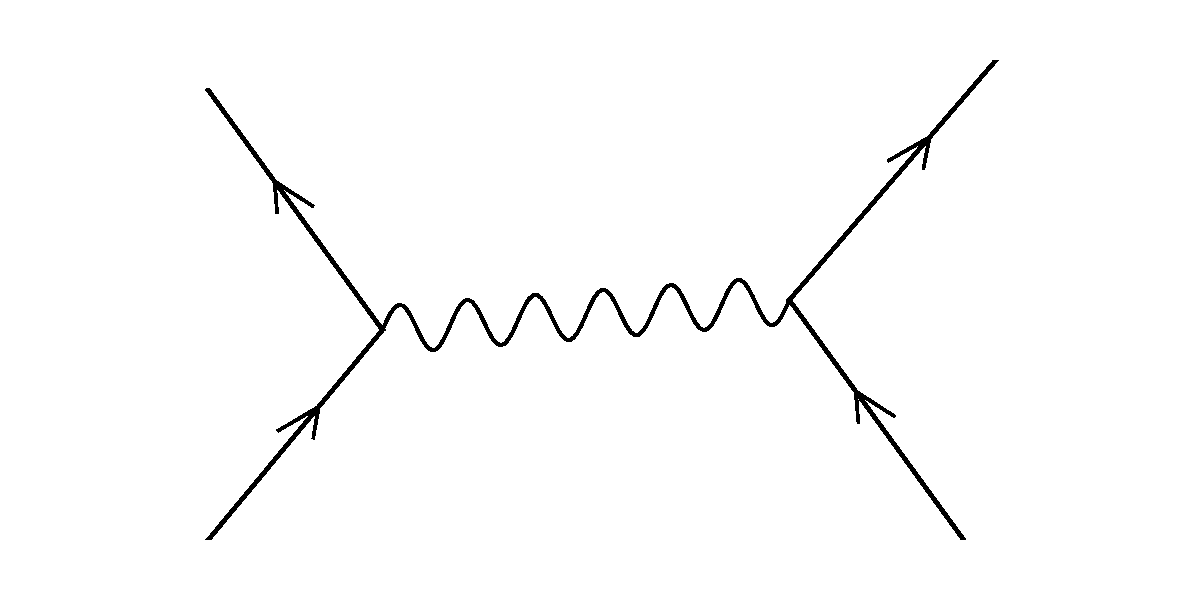
\includegraphics[width=0.7\textwidth]{../img/sq_interaction.pdf}
  \caption{illustration of an $e$-$e$ Interaction were the incoming electrons have initial momentum $k_1$, $k_2$ and spin $\sigma_1$, $\sigma_2$. The interaction $V_q$ causes them to exchange a momentum $q$.}
\end{figure}


The interaction is due to the coulomb repulsion, therefore we can write the interaction term in reciprocal space as 

\begin{equation}
  V_q ~~=~~ \int d^3r e^{i\mathbf{q} \cdot \mathbf{r}} V(\mathbf{r}) 
  ~~=~~ \int d^3r \frac{e^2}{r} e^{i \mathbf{q} \cdot \mathbf{r}} 
  ~~=~~ \frac{4\pi e^2}{q^2}
\end{equation}

Calculating the change in energy resultng from the coulomb interaction between the electrons gives

\begin{equation}
  \frac{E_1}{N} ~~=~~ \frac{\langle \text{FS} | V_\text{el-el} | \text{FS} \rangle}{N} 
  ~~=~~ \frac{1}{2VN} \sum_q \sum_{\mathbf{k}_1, \mathbf{k}_2} \sum_{\sigma_1, \sigma_2}
  \frac{4\pi^2}{q^2} 
  \langle \text{FS} | c^\dag_{\mathbf{k}_1+q} c^\dag_{\mathbf{k}_2-q} c_{\mathbf{k}_2} c_{\mathbf{k}_1} | \text{FS} \rangle  
\end{equation}

\begin{align}
  \langle \text{FS} | c^\dag_{\mathbf{k}_1+q, \sigma_1} c^\dag_{\mathbf{k}_2-q, \sigma_2} c_{\mathbf{k}_2, \sigma_2} c_{\mathbf{k}_1, \sigma_2} | \text{FS} \rangle 
  ~~& =~~ \delta_{\sigma_1 \sigma_2} \delta_{\mathbf{k}_1+q, \mathbf{k}_2} 
  \langle \text{FS} | c^\dag_{\mathbf{k}_1+q} c^\dag_{\mathbf{k}_2-q} c_{\mathbf{k}_2} c_{\mathbf{k}_1} | \text{FS} \rangle \nonumber \\
  ~~& =~~ -\delta_{\sigma_1 \sigma_2} \delta_{\mathbf{k}_1+q, \mathbf{k}_2} 
  \langle \text{FS} | c^\dag_{\mathbf{k}_1+q} c_{\mathbf{k}_1+q} c^\dag_{\mathbf{k}_1} c_{\mathbf{k}_1} | \text{FS} \rangle \nonumber \\
  ~~& =~~ -\delta_{\sigma_1 \sigma_2} \delta_{\mathbf{k}_1+q, \mathbf{k}_2}
  \theta(k_F - |\mathbf{k}_1+q |) \theta(k_F - | \mathbf{k}_1|)
\end{align}


The two delta functions impose the fact that the spin does not change during the interaction and that the momentum is conserved in the process. Furthermore since we can relate $\mathbf{k}_1$ and $\mathbf{k}_2$ we replaced the latter one in the latter operator index.

Here we see the benefit which comes along with this notation. By only using commuation relation for fermion-latter operators we were able to change the rathre complicated expression to one that can easily be integrated.


\begin{figure}
  \centering
  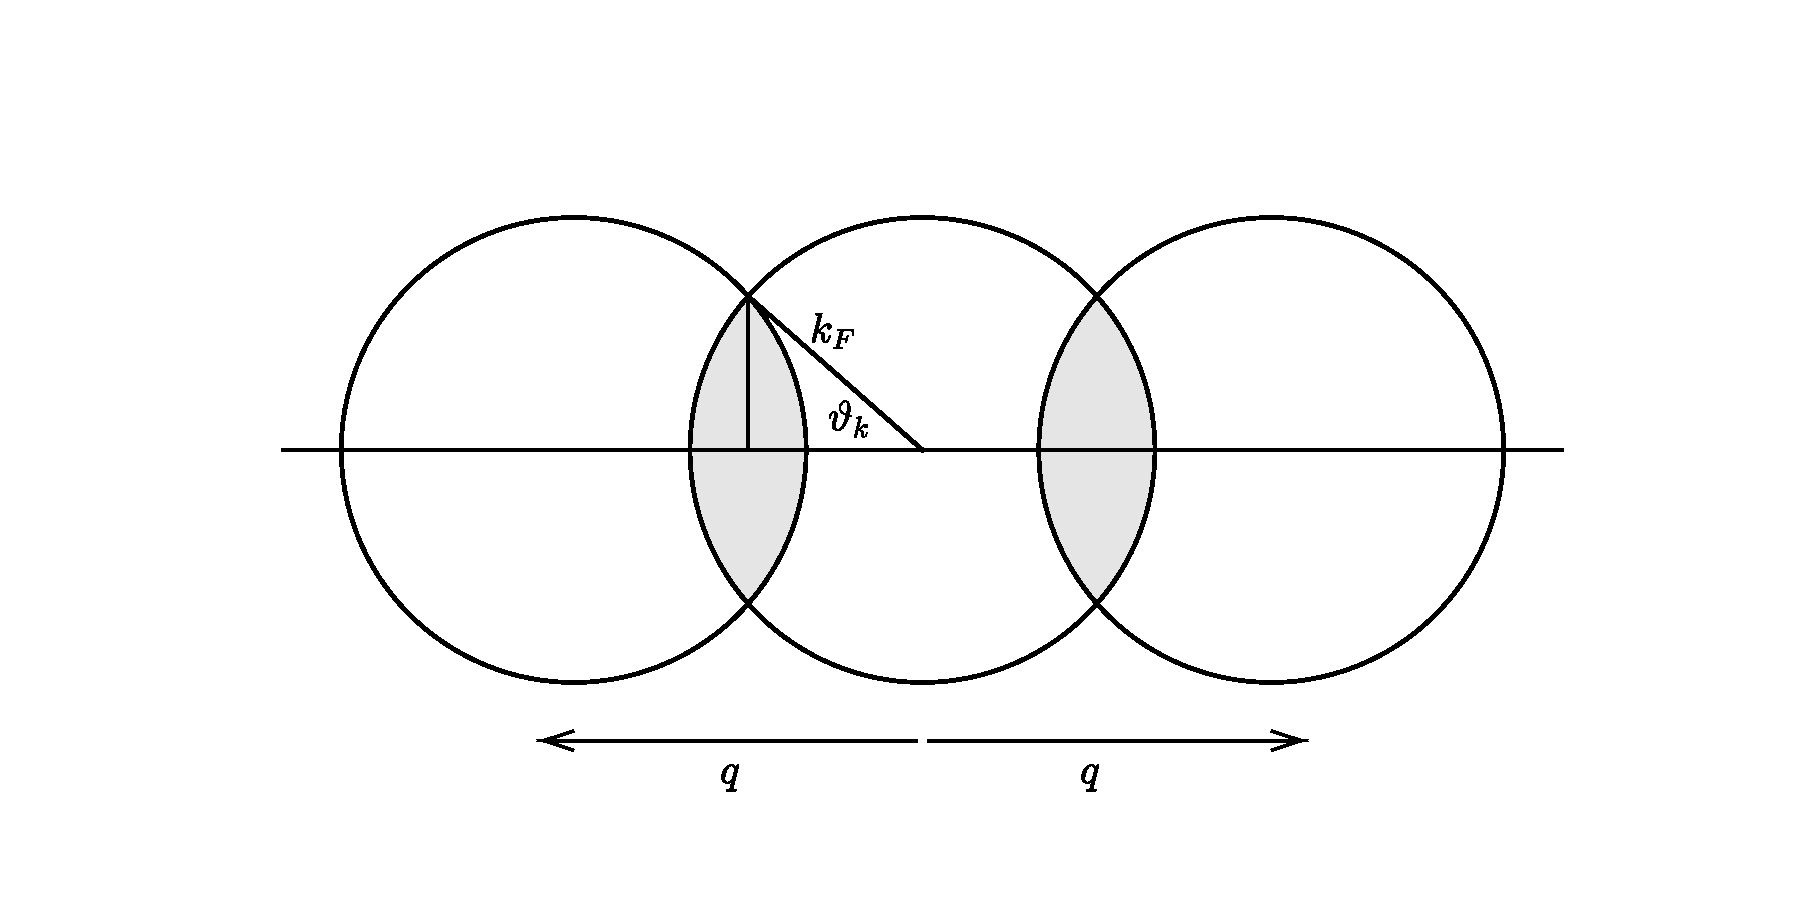
\includegraphics[width=1.0\textwidth]{../img/sq_graph_integration.pdf}
  \caption{illustration of an $e$-$e$ Interaction were the incoming electrons have initial momentum $k_1$, $k_2$ and spin $\sigma_1$, $\sigma_2$. The interaction $V_q$ causes them to exchange a momentum $q$.}
  \label{fig:sq_graph_integration}
\end{figure}

The way to perform this integration can be illustrated graphically \myRef{fig:sq_graph_integration}. 

How to choose the boundaries of integration can be illustrated. 










\subsubsection*{Second Quantization: Free Electron Gas} % 16.10.17 - second part 

$ k_F^3 = 3 \pi^2 n$

$ E_0 = \frac{3}{5} N \epsilon_F$

Bohr Radius: $a_0 = \frac{\hbar}{m e^2}$

\begin{equation*}
\frac{3 \pi^2}{k_F^3} ~~ = ~~ \frac{1}{n} ~~ = ~~ \frac{V}{N} ~~ = ~~ \frac{4\pi}{3} \left(r_S a_0 \right)^3 ~~~~ \Rightarrow ~~~~ r_S = \left( \frac{9\pi}{4} \right)^{1/3} \frac{1}{a_0 k_F}
\end{equation*}

\begin{equation*}
\frac{E_0}{N} ~~ = ~~ \frac{2.21}{r_S^2} \frac{e^2}{2a_0}
\end{equation*}



\subsubsection*{Electron Interaction}

\begin{equation*}
  \frac{E_1}{N} ~~ = ~~ \frac{\bra{FS} V_{el-el} \ket{FS}}{N} ~~ = ~~ 
  - \frac{e^2}{2} \frac{V}{N} \frac{k_F^4}{2 \pi^3} ~~=~~ - \frac{0.916}{r_S} \frac{e^2}{2 a_0}
\end{equation*}


\textcolor{red}{plot - energy minimum at $r_S$}


\begin{equation}
  V_\text{el-el} ~~=~~ \frac{1}{2V} \sum_{\sigma_1 \sigma_2} \sum_{k_1 k_2 q} 
    V_q c_{k_1+q}^\dag c_{k_2-q}^\dag c_{k_2} c_{k_1}
\end{equation}



\subsubsection{Fermi Liquid Theory}

\subsubsection{Electron Tight Binding Model}
% lec-notes 17.10.17
%

%An approximation for an electron wavefunction over the whole crystal can be given as a linear combination of atomic orbitals $\varphi(\mathbf{r})$ of an isolated atom.


An approximation for an electron wavefunction over the whole crystal can be given as

\begin{equation}
  \Psi_k ~~=~~ \sum_j c_{kj} \varphi(\mathbf{r}-\mathbf{r}_j)
\end{equation}

Where $\varphi(\mathbf{r})$ is the ground state wavefunction (atomic orbital) of an electron in the potential $V(\mathbf{r})$ of an isolated atom. This approximation is only valid if the interaction between neighborign atoms is small. The sum goes over all lattice points.


Using

\begin{equation}
  c_{kj} ~~=~~ N^{-1/2} e^{i \mathbf{k} \mathbf{r}_j}
\end{equation}

The factor $N^{-1/2}$ ensures the wavefunction to meet the normalization criterion
We can express the over all wavefunction of an electron in the crystal

\begin{equation} \label{eq:el_wf}
  \Psi_k(\mathbf{r}) 
  ~~=~~ N^{-1/2} \sum_j e^{i\mathbf{k} \mathbf{r}_j} \varphi(\mathbf{r} - \mathbf{r}_j)
\end{equation}


Recalling the \textbf{Bloch Theorem} which states, that the wavefunction of an electron in a periodic potential ($V(\mathbf{r}) = V(\mathbf{r} + \mathbf{a})$) with the periodicity $a$ is given by

\begin{equation} \label{eq:bloch_theorem}
  \phi_k(\mathbf{r}) ~~=~~ u_k(\mathbf{r}) \cdot e^{i\mathbf{k} \mathbf{r}}
\end{equation}

where $u_k(\mathbf{r})$ has the periodicity of the crystal ($u_k(\mathbf{r} + \mathbf{a}) = u_k(\mathbf{r})$). Since the tightbinding ansatz is meant to describe the electrons in a perodic potential, so it also have to be a bloch wave. 


%Applying the Bloch Theorem to our electron wavefunction \refEq{eq:el_wf}, we get
We can show, that our electron wavefunction \refEq{eq:el_wf} fulfills the Bloch criterion


\begin{align}
  \Psi_k(\mathbf{r} + \mathbf{a}) 
  ~~& =~~ N^{-1/2} \sum_j e^{i \mathbf{k} \mathbf{r}_j} \varphi(\mathbf{r} + \mathbf{a} - \mathbf{r}_j) \nonumber \\
  ~~& =~~ N^{-1/2} e^{i\mathbf{k} \mathbf{a}} 
  \sum_j e^{i\mathbf{k} (\mathbf{r}_j - \mathbf{a})} \varphi(\mathbf{r} - (\mathbf{r}_j-\mathbf{a})) \nonumber \\
  ~~& =~~ N^{-1/2} e^{i\mathbf{k} \mathbf{a}}
  \sum_n e^{i\mathbf{k} \mathbf{r}_n} \varphi(\mathbf{r} - \mathbf{r}_n) \nonumber \\
  ~~& =~~ e^{i\mathbf{k} \mathbf{a}} \Psi_k(\mathbf{r})
\end{align}

To get to this result we used the fact, that the summation goes over all lattice points and we therefore can replace the dummy variables $j$ with $n$ by writting $\mathbf{r}_j - \mathbf{a}$ as $\mathbf{r}_n$. This is allowed since $\mathbf{a}$ describes a lattice vector connecting two lattice points.

We can compute now for the energy levels of the tight-binding ansatz

\begin{align}
  \epsilon_k ~~& =~~ \langle \mathbf{k} | H | \mathbf{k} \rangle ~~=~~
  N^{-1} \sum_j \sum_m e^{i\mathbf{k} (\mathbf{r}_j - \mathbf{r}_m)} 
  \langle \varphi_m | H | \varphi_j \rangle 
\end{align}

The double sum can be understood in the following sense: to get the total energy, we have to sum over all the electrons ($\sum_j$), whereas every electron feels a contribution from the potential of every atom in the crystal ($\sum_m$). Since we assum, that the electrons on an atom site mainly feel interactions on the atom site itself and the nearest neightbors, we can neglect all terms with $j \neq m$ of the first sum. We also define $\mathbf{\rho}_m = \mathbf{r}_m - \mathbf{r}_j$

\begin{align} \label{eq:tb_der}
  \epsilon_k ~~& =~~ \sum_m e^{-i\mathbf{k} \mathbf{\rho}_m} \langle \varphi(\mathbf{r}-\mathbf{\rho}_m) | H | \varphi(\mathbf{r}) \rangle \nonumber \\
  ~~& =~~ \langle \varphi(\mathbf{r}) |H| \varphi(\mathbf{r}) \rangle 
  ~+~ \sum_{\rho_m \in \text{NN}} \langle \varphi(\mathbf{r} - \mathbf{\rho_m}) |H| \varphi(\mathbf{r}) \rangle
\end{align}

Defining the coefficients 

\begin{align}
  \epsilon_0 ~~& =~~ \langle \varphi(\mathbf{r}) | H | \varphi(\mathbf{r}) \rangle  ~~=~~
  \int d^3\mathbf{r}\ \varphi^*(\mathbf{r}) H \varphi(\mathbf{r}) \\
  t ~~& =~~ \langle \varphi(\mathbf{r} - \mathbf{\rho_m}) |H| \varphi(\mathbf{r}) \rangle 
  ~~=~~ \int d^3\mathbf{r}\ \varphi^*(\mathbf{r} - \mathbf{\rho_m}) H \varphi(\mathbf{r})
\end{align}

allows us to write \refEq{eq:tb_der} in the abbreviated way

\begin{equation} \label{eq:tb}
  \epsilon_k ~~=~~ \epsilon_0 ~-~ t \sum_{\rho_m} e^{-i\mathbf{k} \mathbf{\rho}_m}
\end{equation}

where $\epsilon_0$, the energy level of the singel atom, defines the position of the energy band and $t$, defined through the overlap of neighboring atoms, defines the width of the energy band.


\subsubsection{Example: cubic lattice structure}

For a cubic lattice structure, taking only the nearest neighbors into account we have to sum over the following lattice sites in the sum of \refEq{eq:tb}

\begin{equation}
  \mathbf{\rho}_m ~~\in~~ \left\{ (\pm a,0 ,0),~ (0, \pm a, 0),~ (0, 0, \pm a) \right\}
\end{equation}

This leads to the following expression for the energy bands

\begin{equation}
  \epsilon_k ~~=~~ E(\mathbf{k}) ~~=~~ \epsilon_0 ~+~ 2t \left[ \cos(k_xa) + \cos(k_ya) + \cos(k_za) \right]
\end{equation}

The position ($\epsilon_0$) and width $W=12t$ is determined by the particulare single atom orbital wavefunction.


%\begin{itemize}
%  \item{The Width of the band is porportional to the strength of the overlap interaction between neighboting atoms.}
%  \item{Tight binding approximation is good for inner electrons. It isn't a good approximation when considering conduction electrons.}
%\end{itemize}
%


\subsection{Charge Ordering}

\begin{figure}
  \centering
  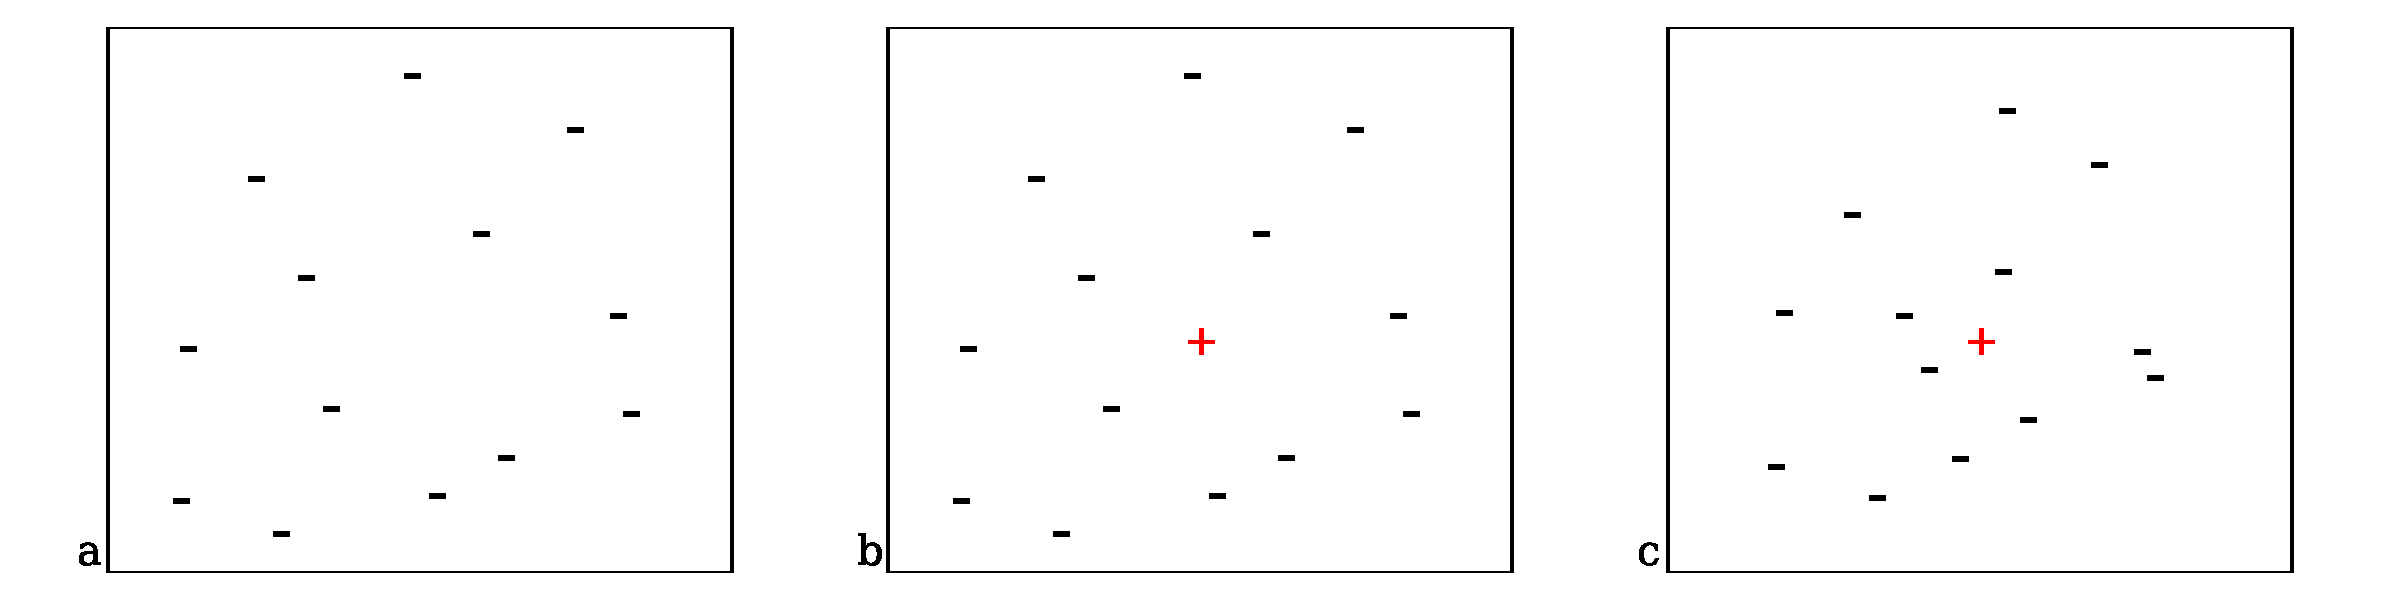
\includegraphics[width=1.0\textwidth]{../img/screening_charge_box.pdf}
  \caption{Sketch of boxes filled with charged particles. \textbf{a.} equally distributed negatively charged particles. \textbf{b.} negativel charges with one positive charge without interactions. \textbf{c.} negative charged particles are attracted by positive charge.}
  \label{fig:screening_charge_box}
\end{figure}

\begin{equation} \label{eq:tot_charge_dens}
  \rho(r) ~~=~~ \rho^\text{Total}(\mathbf{r}) ~~=~~ \rho^\text{Ext}(\mathbf{r}) ~+~ \rho^\text{Ind}(\mathbf{r})
\end{equation}


With the poisson equation we can determine the electric potential $\phi$ produced by the charge density

\begin{align}
  \nabla^2 \phi^\text{Ext} ~~& =~~ -\frac{1}{\epsilon_0} \rho^\text{Ext}(\mathbf{r}) \\
  \nabla^2 \phi	~~& =~~ -\frac{1}{\epsilon_0} \rho(\mathbf{r})
\end{align}


This differential equation can be solved by transforming it to the Fourier space

\begin{align}
  q^2 \phi^\text{Ext}(\mathbf{q}) ~~& =~~ \frac{1}{\epsilon_0} \rho^\text{Ext}(\mathbf{q}) \\
  q^2 \phi (\mathbf{q}) ~~&=~~ \frac{1}{\epsilon_0}  \rho(\mathbf{q})
\end{align}


Using the definitions for the dielectric function $\epsilon$ and the electric susceptibility $\chi$

\begin{align}  \label{eq:screen_dielect}
  \frac{1}{\epsilon(\mathbf{q})} ~~=~~ \frac{\phi(\mathbf{q})}{\phi^\text{Ext}(\mathbf{q})} \\
  \label{eq:screen_suscept}
  \chi(\mathbf{q}) ~~=~~ \frac{\rho^\text{Ind}(\mathbf{q})}{\phi(\mathbf{q})}
\end{align}

We can relate the dielectric function and the susceptebility  by using the formulas for the electric potential from above

\begin{equation}
  \epsilon(\mathbf{q}) ~~=~~ 1 ~-~ \frac{\chi(\mathbf{q})}{\epsilon_0 q^2}
\end{equation}


\subsubsection{Thomas-Fermi Screening}

Calculate $\chi(\mathbf{q})$


Charge density of an electron gas can be expressed in terms of the electron density $n(\mathbf{r})$

\begin{equation}
  \rho_0 ~~=~~ -e n(\mu) ~~~~~~\text{with}~~~~ 
  n(\mu) ~~=~~ \int \frac{d \mathbf{k}}{4\pi^3}\ f_k(\mu)
\end{equation}

The electron density itself is then given as the integral over the Fermi-Dirac distribution. We can write the Schrodinger Equation as 

\begin{equation} \label{eq:screen_hamiltonian}
  -\frac{\hbar^2}{2m} \nabla^2 \Psi_k ~-~ e\phi^\text{Total}\ \Psi_k ~~=~~ \varepsilon_k\ \Psi_k
\end{equation}

Using the Thomas-Fermi approximation in which we assume for the total electric potential to be constant on the length scale of our problem. Then we can write

\begin{equation}
  \varepsilon_k ~~=~~ \frac{(\hbar \mathbf{k})^2}{2m} ~+~ \varepsilon' ~~~~~\text{where}~~~~
  \varepsilon' ~=~ e\ \phi(\mathbf{r})
\end{equation}

With this new expression for the electron energy $\varepsilon_k$ we are able to write an expression for the electron density $n(\mathbf{r})$ of the whole system

\begin{align}
  n^\text{Total} ~~& =~~ \int \frac{d \mathbf{k}}{4\pi^3} \left(e^{(E_k + \mu)/k_BT} ~+~ 1 \right)^{-1} \nonumber \\
  ~~& =~~ \int \frac{d \mathbf{k}}{4\pi^3} \left(e^{(\frac{(\hbar \mathbf{k})^2}{2m} + \varepsilon' + \mu)/k_BT} ~+~ 1 \right)^{-1} 
  ~~=~~ n(\mu + \varepsilon')
\end{align}


As we know from \refEq{eq:tot_charge_dens} the induced charge density is given as the difference between the total charge density $n(\mathbf{r}$ and the external charge density $n_0$. Therfore we can write

\begin{equation} \label{eq:thomas_fermi}
  \rho^\text{Ind}(\mathbf{r}) ~~=~~ -e \left[ n(\mu + \varepsilon') ~-~ n(\mu) \right] 
  ~~=~~ -e \cdot \varepsilon'\ \frac{dn}{d\mu}
\end{equation}

The difference of the two electron density was replaced by de derivative by using the defintion of derivaties $df/dx = (f(x+\Delta x) - f(x))/\Delta x$.
\refEq{eq:thomas_fermi} is known as the basic equation of the Thomas-Fermi Theory. Replacing $\varepsilon'$ by the electric potential again and Fourier transforming \refEq{eq:thomas_fermi} gives

\begin{equation}
  \rho^\text{Ind}(\mathbf{q}) ~~=~~ -e^2 \frac{dn}{d \mu} \phi(\mathbf{q})
\end{equation}

Comparing this to \refEq{eq:screen_suscept} we found for the susceptibility and the dielectric function

\begin{equation} \label{eq:thomas_fermi_function}
  \chi ~~=~~ -e^2 \frac{dn}{d \mu} ~~~~~~\text{and}~~~~~~~ 
  \epsilon(\mathbf{q}) ~~=~~ 1 + \frac{e^2\ dn/d\mu}{\epsilon_0 q^2}
\end{equation}

It is important to note that the susceptibility does here not depend on the wavevector $\mathbf{q}$. This is a result of our approximation that $\phi(\mathbf{r})$ does not vary much over $\mathbf{r}$.


\subsubsection{Thomas-Fermi Wavevector}

Defining the Thomas-Fermi Wavevector $\mathbf{k}_0 ~~=~~ \frac{e^2 dn/d\mu}{\epsilon_0}$ allows us to write \refEq{eq:thomas_fermi_function} as 

\begin{equation} \label{eq:screening_dielect_new}
  \epsilon(\mathbf{q}) ~~=~~ 1 ~+~ \frac{\mathbf{k}_0^2}{\mathbf{q}^2}
\end{equation}

From this expression it is visible that we can define a characteristic lengthscale of the electron screening. This lengthscale is given as $1/\mathbf{k}_0$ and we refer to it as \textbf{Thomas-Fermi Screening Length}. For copper we have a screening length of $1/\mathbf{k}_0 = \SI{0.55}{\AA}$.


\begin{figure}
  \centering
  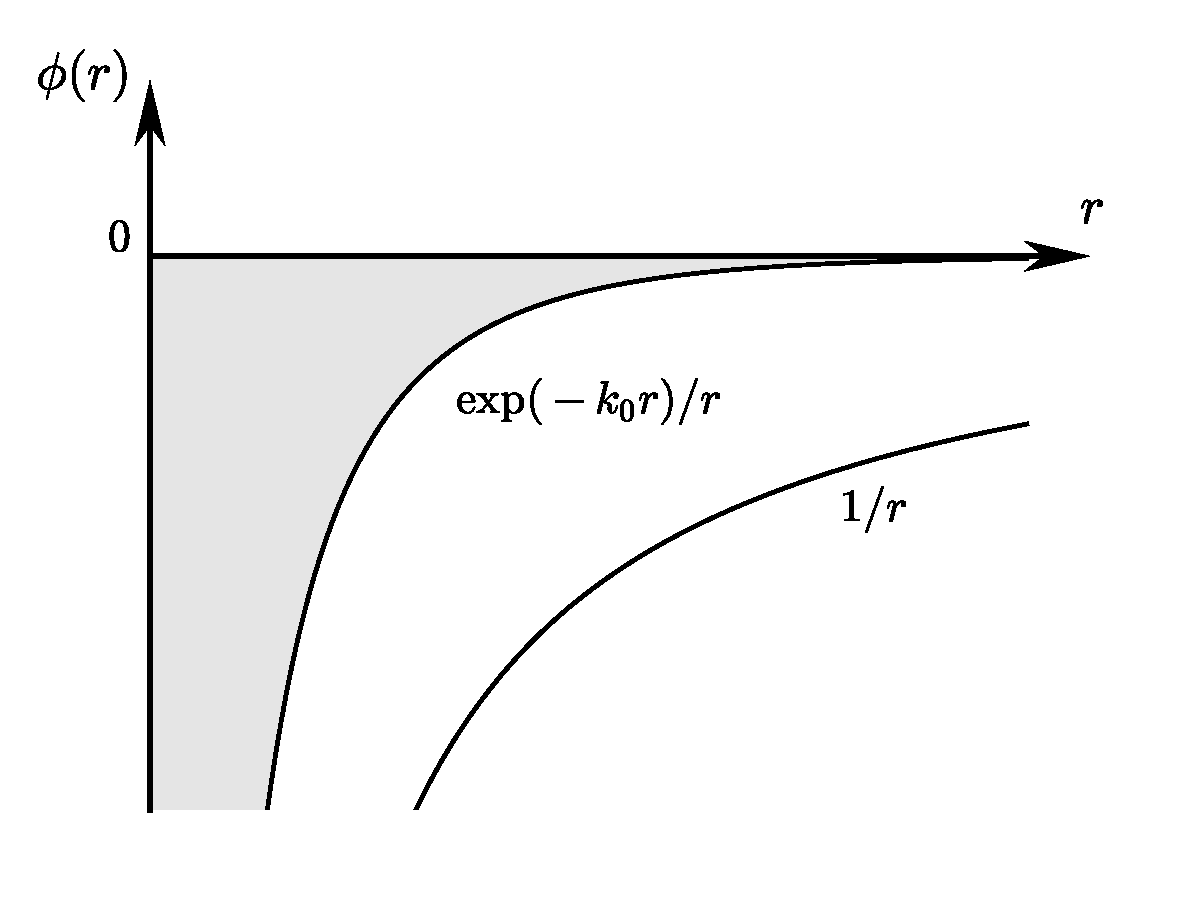
\includegraphics[width=0.6\textwidth]{../img/screening_yukawa.pdf}
  \caption{Illustration of bare coulomb potential ($r^{-1}$) and the Yukawa potential.}
  \label{fig:screening_yukawa}
\end{figure}



\subsubsection{Example: Coulomb Potential}

Looking at a point charge $Q$ placed in a sea of conduction eletrons, as illustrated in \myRef{fig:screening_charge_box}.b we can express the externel potential generated from the point charge as $\phi^\text{Ext}(\mathbf{r}) = Q/r$ with its Fouriere transform  $\phi^\text{Ext}(\mathbf{q}) = 4\pi\ Q/q^2$. Rearanging \refEq{eg:screnn_dielect} and replacing the dielectric function by \myRef{eq:screening_dielect_new}, we obtain

\begin{equation}
  \phi(\mathbf{q}) ~~=~~~\frac{\phi^\text{Ext}(\mathbf{q}}{\epsilon(\mathbf{q}} 
  ~~=~~ \frac{4\pi\ Q}{q^2 + k^2_0}
\end{equation}

Fourier transform this back to real space leads to the well known \textbf{Yukawa Potential} 

\begin{equation}
  \phi(\mathbf{r}) ~~=~~ Q \frac{e^{-i k_0 r}}{r}
\end{equation}

The difference between the Coulomb- and Yukawa potential are displayed in \myRef{fig:screening_yukawa}. The screening effect added point charge by the surrounding negative charges is clearly visible in the faster convergence to zero of the Yukawa Potential. The screening also weakens the longe range interaction of the charges in the solid.


\subsection{Lindhard Potential}

A more sophisticated approach is provided by the Lindhard Theory from which the Thomas-Fermi screening is a special case ($\mathbf{q} \ll \mathbf{k}_0$). The basic idea here is to find a solution for the Schrodinger equation by treating the electrical potential $\phi^\text{Ext}(\mathbf{r})$ introduced by the external charge as a pertubation, which allows us then to use the methodology of pertubation theory.

As we know, the charge density for one electron with momentum $\mathbf{k}$ is given as $\rho_\mathbf{l}(\mathbf{r}) = e|\psi_\mathbf{k}(\mathbf{r})|^2$. Describing the the overall charge density of a crystal, assuming it is in its groundstate we have to sum the one electron charge density multiplied with the fermi function $f_\mathbf{k}$ over all momenta $\mathbf{k}$

\begin{equation} \label{eq:lindh_charge}
  \rho(\mathbf{r}) ~~=~~ -e \sum_\mathbf{k} f_\mathbf{k} | \Psi_\mathbf{k}(\mathbf{r}) |^2
\end{equation}

%Assuming the additional term $e\phi$ in our Hamiltonian (\refEq{eq:screen_hamiltonian}), introduced throught the external charge, can be treated as a pertubation, we can express the one electron wavevector $\psi_\mathbf{k}$ as

As mentioned above, assuming the term $e\phi$ as petubation, we can express the electron wavevector $\psi_\mathbf{k}$ as 

\begin{equation} \label{eq:lindh_wf}
  \psi_\mathbf{k} ~~=~~ | \mathbf{k}_0 \rangle ~+~ \sum_\mathbf{k}' \frac{\langle \mathbf{k}' | e\phi | \mathbf{k}_0 \rangle}{\varepsilon_{\mathbf{k}_0} - \varepsilon_{\mathbf{k}'}}
\end{equation}


To plug our ansatz for $\psi_\mathbf{k}$ into \refEq{eq:lindh_charge} we evaluate first

\begin{align} \label{eq:lindh_wf_squared}
  | \psi_\mathbf{k} |^2 ~~& =~~ \left( |\mathbf{k}_0 \rangle ~+~ \sum_{\mathbf{k}'}\ ...\ |\mathbf{k}' \rangle \right) \left( \langle \mathbf{k}_0 | ~+~ \sum_{\mathbf{k}'}\ ...\ \langle \mathbf{k}' | \right) \nonumber \\
  ~~& =~~ \langle \mathbf{k}_0 | \mathbf{k}_0 \rangle ~+~ 
  \underbrace{\sum_{\mathbf{k}'}\ ...\ \langle \mathbf{k}_0 | \mathbf{k}' \rangle}_{A} ~+~ 
  \underbrace{\sum_{\mathbf{k}'}\ ...\ \langle \mathbf{k}_0 | \mathbf{k}' \rangle}_{B} ~+~ \OO(2)
\end{align}


Using this equation we can write the charge density \refEq{eq:lindh_charge} in the following way

\begin{equation}
  \rho^\text{Ind}(\mathbf{r}) ~~=~~ -e \sum_{\mathbf{k}} f_\mathbf{k} (A+B)
\end{equation}


Simplifying this equation is easier in Fourier space

\begin{equation}
  \rho^\text{Ind}(\mathbf{q}) ~~=~~ \int \rho^\text{Ind}(\mathbf{r})\ e^{i\mathbf{q} \mathbf{r}} d^3\mathbf{r} 
  ~~=~~ -e \int d^3\mathbf{r}\ \sum_\mathbf{k} f_\mathbf{k}\ (A+B) \cdot e^{i\mathbf{q} \mathbf{r}}
\end{equation}

Calculating the Fourier transform for the two variables $A$ and $B$ works similar. We set $\mathbf{k}' = \mathbf{k} + \mathbf{q}$. This gives

\begin{align}
  -e \int d^3\vc{r}\ \sum_\vc{k} f_\vc{k}\ A \cdot e^{i\vc{q}\vc{r}} 
  ~~& =~~ -e \int d^3 \vc{r} \sum_{\vc{k}'} \sum_\vc{k} f_\vc{k}
  \frac{\overbrace{\langle \vc{k}-\vc{q}| e\phi(\vc{r})|\vc{k}\rangle}^{\text{FT of } \phi(\vc{r})}}{\varepsilon_\vc{k} ~-~ \varepsilon_{\vc{k}-\vc{q}}} \nonumber \\
  ~~& =~~ -e^2 \sum_{\vc{k}'} \sum_\vc{k} \frac{f_\vc{k}\ \phi(\vc{q})}{\varepsilon_\vc{k} - \varepsilon_{\vc{k}+\vc{q}}}
\end{align}


The same goes for the variable $B$

\begin{equation}
  -e \int d^3\vc{r}\ \sum_{\vc{k}'} f_\vc{k}\ B \cdot e^{i\vc{q}\vc{r}} 
  ~~=~~ -e^2 \sum_{\vc{k}'} \sum_\vc{k} \frac{f_{\vc{k}'+\vc{q}}\ \phi(\vc{q})}{\varepsilon_{\vc{k}'+\vc{q}} - \varepsilon_{\vc{k}'}}
\end{equation}



With these expressions for $A$ and $B$ and the definition of the electric susceptibility $\chi(\vc{q})$ (\refEq{eq:screen_suscept} we can write

\begin{equation}
  \chi(\vc{q}) ~~\propto~~ \int \frac{d^2 \vc{k}}{(2\pi)^n}\ \frac{f_\vc{k} - f_{\vc{k}+\vc{q}}}{\varepsilon-\vc{k} - \varepsilon_{\vc{k}+\vc{q}}}
  ~~~~~~~~\text{with the dimensionality}~ n \in \{1,2,3\} 
\end{equation}


By knowing the band structure one can now calculate $\chi{\vc{q})}$. In this way one is able to experminentaly measure the screening potential.



\textcolor{red}{picture lindhard susceptibility for different dimensions}

%Considering the analogy between $(\phi^\text{Ext}, \phi^\text{Total})$ and the macroscopic quantities $(\mathbf{D}, \mathbf{E})$ we can write a similar equation as it is known for $\mathbf{D}$ and $\mathbf{E}$.

%\begin{equation} \label{eq:dielectric_relation}
%  \phi^\text{Ext}(\mathbf{q}) ~~=~~ \epsilon(\mathbf{q})\ \phi^\text{Total}(\mathbf{q})
%\end{equation}




%=======================================================================
% Magnetism
%=======================================================================

\chapter{Magnetism}

\section{Paramagnetism}

\subsubsection{Magnetic Moment}

\textcolor{red}{insert picture - magnetic moment}

If $\vec{A}$ is the area inside the loop and $I$ the current, the magnetic moment can be written as

\begin{equation} \label{eq:mag_mom}
  \vec{\mu} ~~=~~ I \vec{A}
\end{equation}


\subsubsection{Example: Hydrogen Atom}

\textcolor{red}{insert picture - hydrogen atom and orbiting electron}

The magnetic moment of a hydrogen atom can be described semi-classically by assuming the electron to be on a fixed trajectory orbiting the hydrogen nucleus with constant radius $r$ and velocity $v$. The current $I$ produced by the moving electron can be written as $I = -e/\tau$ with the orbital period $\tau = 2\pi r/v$. For the loop area we use the formula $A= \pi r^2$. This leads the magnetic moment to be

\begin{equation} \label{eq:dev_mag_mom}
  \mu ~~=~~ \frac{-e v \pi r^2}{2 \pi r} ~~=~~ \frac{-evr}{2} ~~=~~ \frac{-e m v r}{2m}
\end{equation}

We can identify the classical definition of the angular momentum  $\vec{l} = \vec{r} \times m \vec{v}$ in the numerator. Taking the quantisation of angular momentum $|\hat{l}| = n \hbar$ in quantum mechanics into account we can rewritte expression \ref{eq:dev_mag_mom} for $n=1$

\begin{equation} \label{eq:bohr_mag}
  \mu ~≃ ~~ \frac{-e \hbar}{2m} ~~ \equiv ~~ -\mu_B
\end{equation}

Which we define as the Bohr magneton $\mu_B$.


\subsubsection{Magnetic Moment of Atoms}

The total angular momentum in an atom is given as the sum of total orbital angular Momentum $\hat{L}$  and total spin angular momentum $\hat{S}$

\begin{equation}
  \hat{J} ~~≃~~ \hat{L} ~+~ \hat{S}
\end{equation}

\subsubsection{Magnetisation}

Considering a solid with $N$ atoms each having a magnetic moment $\vec{\mu}$. We define the magnetization as 

\begin{equation}
  \vec{M} ~~\equiv~~ \frac{\text{Magnetic moment}}{\text{Volume}}
\end{equation}

\begin{figure}
  \centering
  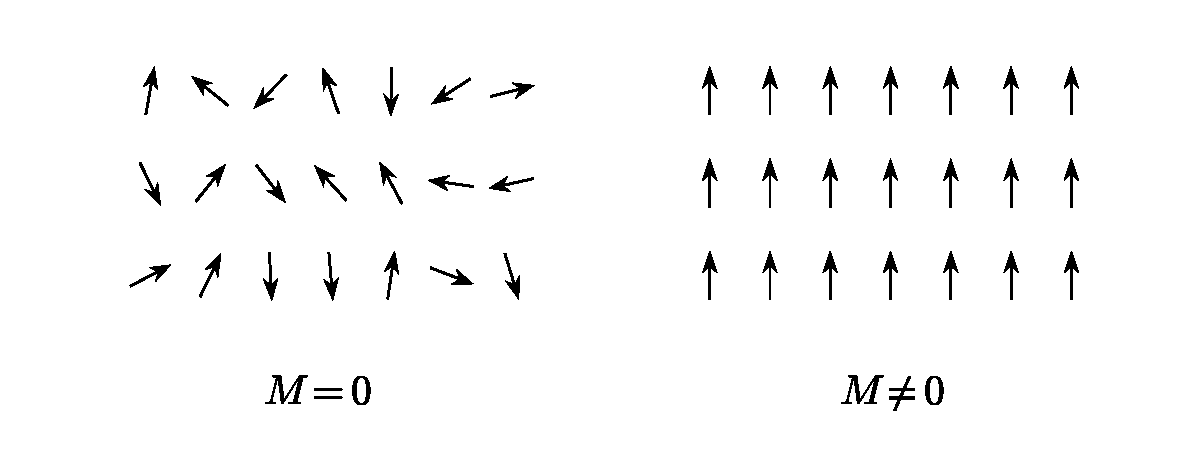
\includegraphics[width=0.8\linewidth]{../img/mag_in_solid.pdf}
  \caption{hohohoh}
\end{figure}

\subsubsection{Magnetic Moment in a $\vec{B}$-Field}


From classical electrodynamics we know that the potential energy $E$ of a magnetic moment $\vec{\mu}$ in a magnetic field $\vec{B}$ is described as

\begin{equation}
  E ~~=~~ - \vec{\mu} ~\cdot~ \vec{B}
\end{equation}

To get a feeling for the order of magnitudes of magnetic energy of atomic scale we 

\begin{equation*}
  \mu_B ~\times~ 1 \text{Tesla} ~~\simeq~~ \SI{0.05}{meV}
\end{equation*}

This is comparable to the energy one has to put into a system to increase its temperature by \SI[mode=text]{1}{K} ($ k_B \cdot \SI{1}{K} ~~\simeq~~ \SI{0.084}{meV}$).


\subsubsection{Magnetic susceptibility}

\begin{equation} \label{eq:mag_suscept}
  \chi ~~≃~~ \frac{\mu_0 \vec{M}}{\vec{B}}
\end{equation}

We can look at the magnetic susceptibility $\chi$ as response function. $\chi$ describes the response of the system $\vec{M}$ when exposed to an external changing field $\vec{B}$.
To simplify things in the calculations we will make the following constraints on $\vec{B}$.

\begin{align*}
  \vec{B} \text{is static} ~~~~ &  \Rightarrow  ~~~~ \text{no time dependence}\\
  \vec{B} \text{is homogeneous} ~~~~ & \Rightarrow  ~~~~ \text{no depencence on}\ \vec{r}
\end{align*}


The definition of the susceptibility allows us now to classify materials depending on how the respond to an external magnetic field. We calc materials to be \textit{paramagnetic} if they align there spin parallel to the applied $\vec{B}$-Field. This is the case if $\chi > 0$. On the contrary we refer to materials as \textit{diamagnetic} if their inner magnetic moments align anti-parallel in respect to an applied field $\vec{B}$. This results in a negativ value for the susceptibility $\chi < 0$.

In reality, the response of systems is composed of multiple differenent responses which can have different origins.

\begin{equation}
  \chi_{total} ~~≃~~ \chi_\text{paramagnetic} ~+~ \chi_\text{diamagnetic} ~+~ ...
\end{equation}

Paramagnetism and diamagnetism can also have different origins. For example:

\begin{align*}
  \chi_\text{paramagnetic} ~~& ≃~~ \chi_\text{Langevin} ~+~ \chi_\text{Van Vleck} ~+~ \chi_\text{Pauli} ~+~ ....\\
  \chi_\text{diamagnetic} ~~& ≃~~ \chi_\text{electronic} ~+~ \chi_{superconductivity} ~+~ ...  
\end{align*}



\subsubsection{Diamagnetism}

\textcolor{red}{insert picture - loop current to illustrate lens law}

To symbolize diamagnetic behaviour we recall lens law. It states, that a a changing magnetic field induces a current which creates for itself a magnetic field that points in the opposit direction as the initial magnetic field change. In that way the system tries to compensate the externaly induced field changes.

To describe that, we use \ref{eq:mag_mom}, with the area $\vec{A} = \pi <r^2>$ and the current $I = -Z e/ \tau$ with the number of electrons $Z$ per atom and the orbit period $\tau$. expression the orbit period in terms of the \textit{cyclotron frequency} $\omega = eB/2m$ shows the dependency on the magnetic field.

\begin{equation}
  \tau ~~=~~ \frac{2\pi}{\omega} ~~=~~ \frac{4\pi m}{e B}
\end{equation}

Putting everything together we get the following expression to approximate the magnetic moment of a diamagnet

\begin{equation} \label{eq:mag_mom_diamag}
  \vec{\mu} ~~=~~ -\frac{Z e^2 B}{4\pi m} \pi <r^2> ~~=~~ -\frac{Ze^2B}{4m} <r^2>
\end{equation}

The magnetisation of a macroscopic material can be written as the sum over all the magnetic moments of its atoms resulting in

\begin{equation}
  \vec{M} ~~=~~ \mu_0 N \vec{\mu}
\end{equation}

where $N$ denotes the number of atoms per volume. Recalling \ref{eq:mag_suscept}, we find for the diamagnetic susceptibility caused by electrons

\textcolor{red}{compare formula with wikipedia. probably wrong by a prefactor}

\begin{equation}
  \chi_\text{Diamagnetic} ~~=~~ -\frac{\mu_0 N e^2 <r^2> Z}{4m}
\end{equation}


\subsubsection{Simplest Case: $e^-$ only}

Consider a system consisting of atoms with only one electron

\begin{equation}
  \rightarrow ~~ \hat{L} ~~=~~0, ~~~~ \hat{S} ~~≃~~ 1/2 ~~~~~~~~~\Rightarrow ~~ \hat{J} ~~=~~ 1/2
\end{equation}

Further more we asume for the spin g-factor $g \simeq 2$ (not proved). This system has only to states: \textit{spin-up} and \textit{spin-down}.


Consider the energy of these two states leads to

\begin{equation}
  E ~~=~~ - \vec{\mu} \cdot \vec{B} ~~=~~ \pm \mu_B \cdot |\vec{B}|
\end{equation}

\textcolor{red}{ vector diagram nergy consideration of magnetic moment in B-field}

As stated before, the Energy resulting from magnetic moments of the order of magnituted of a bohr magneton $\mu_B$ to magentic fields to several Tesla are in the same the energy range of some Kelvin ( some $k_B T$). Therefore we use Boltzman statistics to describe the \textbf{population distribution} of the system. The probability of energy level $E_1$ to be populated can be written as

\begin{equation}
  p_\alpha ~~=~~ \frac{e^{\beta E_\alpha}}{\mathcal{Z}} ~~=~~ \frac{e^{\beta E_\alpha}}{e^{\beta E_1} + e^{\beta E_2}}, ~~~~ \text{with} ~~ \alpha = \{1,2\}
\end{equation}


where $\beta = 1/k_BT$ and the partition function $\mathcal{Z} = \sum_i e^{\beta E_i}$. 


\begin{equation}
  p_1 ~~=~~ \frac{e^{ \beta E_1}}{e^{\beta E_1} + e^{-\beta E_1}}, ~~~~ 
  p_2 ~~=~~ \frac{e^{-\beta E_1}}{e^{\beta E_1} + e^{-\beta E_1}}
\end{equation}

This has to be equatl to $p_1 = N_1/N$ and $p_2 = N_2/N$ with $N_1$ ($N_2$) being the number of electrons in the energy state $E_1$ ($E_2$) and $N = N_1 + N_2$ being the total number of electrons in the system. Futhermore we subtitute $\Bar{x} = \beta E_1 = \mu_B b/k_B T$.

\textcolor{red}{plots energy level polulation}


The magnetisation $M$ can now be written as the difference in the number of electrons with opposite magnetic moment

\begin{align}
  M ~~& =~~ (N_1 - N_2) \mu_B ~~=~~ N \mu_B (\frac{N_1}{N} - \frac{N_2}{N}) ~~=~~ 
  N \mu_B \left( \frac{e^{\Bar{x}} - e^{-\Bar{x}}}{e^{\Bar{x}} + e^{-\Bar{x}}} \right) \nonumber \\
  M ~~& =~~ N \mu_B \tanh(\Bar{x})
\end{align}


Looking at the case $\Bar{x} \ll 1$, which stands for having large Temperatures and/or low magnetic fields. We get for the magnetisation

\begin{equation}
  M ~~\simeq~~ N \mu_B \Bar{x} ~~=~~ N \frac{\mu_B^2 B}{k_B T}
\end{equation}

With the help of this equation we can now write down an expression for the paramagnetic susceptibility for (large temperature or low magnetic fields)

\begin{equation}
  \chi_\text{paramagnet} ~~=~~ \frac{N \mu_B^2}{k_B T} 
\end{equation}

We refer to this formula as \textit{Curie law} and we call the introduced constant $C = N \mu_B^2/k_B$ \textit{Curie-constant}.


\subsection{How to fill the valence shell}

\subsubsection{Hund's rules}

The hund's rules provide simply rules which give an idea about the total spin-, total orbital- and total angular momentum of an atom in its ground state

\begin{enumerate}
  \item{Maximize $S$ to minimize the Coulomb energy}
  \item{Maximize $L$ to minimize Coulomb repulsion}
  \item{ $J=|L-S|$ for less than half filling and $J=|L+S|$ for more than half filling.}
\end{enumerate}

\subsubsection{Crystal field effects}

Atoms arranged in a lattice feel the presence of the atoms around. This happens in a way, that the valence electrons of the atom under consideration are experiencing the electric field from the ligands surrounding the atom. That causes the energy degenerecy, apparent in a free atom, to be lifted. This splitting of energy levels has impact on the occupation of the different orbitals when "filling" the atom with electrons.
For studying this effect now we will consider the valence electrons to partially fill the $3d$-orbital because this is also the case in a variety of materials in nature. Partially filled $3d$-bands can especially be found in the \textit{Transition metals}. 
 We now exemplify that at at systems with ligands arranged octahedraly and tetragonal. 


\subsubsection{Octahedral crystal environment}



\subsubsection{Tetrahedral crystal environment}


\subsubsection{Variation of crystal field environment}


\subsubsection{Jahn-Teller Distortion}

\textcolor{red}{complete this subsubsection with infos from lecture notes}


\subsubsection{Resonant inelastic x-ray scattering (RIXS)}


%===============================================================================================================
% Feromagnetism
%===============================================================================================================

\section{Ferromagnetism}

\subsection{H\textsubscript{2} Molecule}

\subsubsection{Wave Function Considerations}

\begin{align}
  \Psi^{Total}(\text{2 Electrons})   ~~~~ \rightarrow ~~~~ \text{Antisymmetric}\\
  \Psi^{Total}(\vec{r}_1, \vec{r}_2) ~~~~ = ~~~~ - \Psi^{Total}(\vec{r}_2, \vec{r}_1)
\end{align}


\begin{align}
  \Psi_A ~~~~ = ~~~~ \psi_\alpha(\vec{r}_1) \psi_\beta(\vec{r}_2) ~~ - ~~ \psi_\alpha(\vec{r}_2)\psi_\beta(\vec{r}_1)\\
  \Psi_S ~~~~ = ~~~~ \psi_\alpha(\vec{r}_1) \psi_\beta(\vec{r}_2) ~~ + ~~ \psi_\alpha(\vec{r}_2)\psi_\beta(\vec{r}_1)
\end{align}



Consider now spin wave function:

\begin{equation}
  \chi_S ~~ = ~~ \chi_{Symmetric} ~~ = ~~ \left\{ 
  \begin{array}{ll}
    | \uparrow_\alpha \downarrow_\beta \rangle &~~ | 1,1 \rangle\\
    \left( | \uparrow \downarrow \rangle ~+~ | \downarrow \uparrow \rangle \right)/ \sqrt{2} &~~ | 1,0 \rangle\\
    | \downarrow_\alpha \uparrow_\beta \rangle &~~ | 1,-1 \rangle
  \end{array}\right.
\end{equation}

\begin{equation}
  \chi_A ~~ = ~~ \chi_{Antisymmetric} ~~ = ~~ 
  \begin{array}{ll}
    \left(| \uparrow \downarrow \rangle ~-~ | \downarrow \uparrow \rangle \right) / \sqrt{2} &~~ | 0,0 \rangle 
  \end{array}
\end{equation}

Where to the $\chi_S$ is refered to as \textbf{Triplet state} and to the wave function $\chi_A$ is refered to as textbf{Singlet state}.


\subsubsection{Quantum mechanical Spin-Operators}

Recalling that $\hat{S}^2 |S,m \rangle = S(S+1) | S,m \rangle$ we get for the eigenvalues of $\hat{S}^2_\alpha$ and $\hat{S}^2_\beta$

\begin{align}
  \hat{S}^2_\alpha |S_\alpha,m\rangle ~~ & = ~~ S_\alpha (S_\alpha+1) |S_\alpha,m\rangle ~~ & = ~~ 3/4\\
  \hat{S}^2_\beta  |S_\beta,m\rangle ~~ & = ~~ S_\beta  (S_\beta+1)  |S_\beta,m\rangle ~~ & = ~~ 3/4
\end{align}


\begin{equation}
  \hat{S} ~~=~~ \hat{S}_\alpha ~+~ \hat{S}_\beta ~~~~ \Rightarrow ~~~~ 
  \hat{S}^2 ~~=~~ \hat{S}^2_\alpha ~+~ \hat{S}^2_\beta ~+~ 2 \hat{S}_\alpha \hat{S}_\beta ~~~~ \Rightarrow ~~~~
  \hat{S}_\alpha \cdot \hat{S}_\beta ~~=~~ \frac{\hat{S}^2 - \hat{S}^2_\alpha - \hat{S}^2_\beta}{2}
\end{equation}


Calculating $\langle \hat{S}_\alpha \cdot \hat{S}_\beta \rangle$ leads to $1/4$ for $\chi_S$ and $-3/4$ for the $\chi_A$ case.


\subsubsection{Consider weak Coulomb interaction}


\begin{equation}
  H ~~=~~ H_\text{signel-H} ~+~ H_\text{int} ~~=~~ H_0 ~+~ H_\text{int}
\end{equation}

Where the interaction Hamiltonian $H_\text{int}$ inlcudes the proton-proton, electron-electron, proton 1 - electron 2 and electron 1 - proton 2 interactions.

\begin{equation}
  H_{int} ~~=~~ \frac{e^2}{d_{pp}} ~+~ \frac{e^2}{d_{ee}} ~-~ \frac{e^2}{d_{ep}} ~-~ \frac{e^2}{d_{pe}}
\end{equation}

Here $d_{pp}$ stands for the proton-proton distance, $d_{ee}$ for the electron-electron distance.
Furthermore contains $H_\text{single-H}$ both Hamiltonians of the single hydrogen atoms

\begin{equation}
  H_\text{single-H} ~~=~~ H_{H_1} ~+~ H_{H_2} ~~=~~ 
  \frac{\hbar}{2m} \left( \nabla^2_\alpha + \nabla^2_\beta \right) ~-~ 
  \left(\frac{e^2}{d_{p_\alpha e_\alpha}} + \frac{e^2}{d_{p_\beta e_\beta}} \right)
\end{equation}


%\begin{equation}
%  E_+ ~=~E_S ~~=~~ \langle \Psi_S | H_\text{int} | \Psi_S \rangle ~~=~~
%  \int \left( \psi_\alpha \psi_\beta + \psi_beta \psi_\alpha \right)^* H_\text{int} 
%  \left( \psi_alpha \psi_\beta + \psi_\beta \psi_\alpha \right) d^3r
%\end{equation}

\begin{equation}
  E_+ ~=~E_S ~~=~~ \langle \Psi_S | H_\text{int} | \Psi_S \rangle ~~=~~
  \int ( \psi_\alpha \overbracket[0.5pt][3pt]{ \psi_\beta + \psi_\beta \overbracket[0.5pt][3pt]{ \psi_\alpha )^* H_\text{int} 
  ( \psi_\alpha }^{J_2} \psi_\beta + \psi_\beta}^{J_1}  \psi_\alpha ) d^3r
\end{equation}



\begin{equation}
  E_- ~=~E_A ~~=~~ \langle \Psi_S | H_\text{int} | \Psi_S \rangle ~~=~~
  \int ( \psi_\alpha \overbracket[0.5pt][3pt]{ \psi_\beta - \psi_\beta \overbracket[0.5pt][3pt]{ \psi_\alpha )^* H_\text{int} 
  ( \psi_\alpha }^{J_2} \psi_\beta - \psi_\beta}^{J_1} \psi_\alpha ) d^3r
\end{equation}

% connect different terms with each other
% https://tex.stackexchange.com/questions/265787/connecting-parts-of-equations-with-lines

By defining $C \equiv C_1+C_2$ and $J \equiv J_1+J_2$ one can write the the two energies as

\begin{equation}
  E_\pm ~~=~~ C ~\pm~ J
\end{equation}

Furthermore for the difference of the singlett- and triplett energy we get

\begin{equation}
  E_+ - E_- ~~=~~~2J \int \psi^*_\alpha \psi^*_\beta H_\text{int} \psi_\alpha \psi_\beta d^3r
\end{equation}

From this equatoin we can associate the introduced variable $J$ as the \textbf{Exchange Integral}.

\begin{equation}
  J ~~=~~ \frac{E_+-E_-}{2} ~~=~~ \int \psi^*_\alpha \psi^*_\beta H_\text{int} \psi_\alpha \psi_\beta d^3r
\end{equation}


\subsubsection{What is H\textsuperscript{Spin}\textsubscript{int}}

\begin{equation}
  E_\pm ~~=~~ C ~\pm~ J ~~=~~ C ~+~ J/2 ~+~ 2J ~+~ \cdot \rangle \hat{S}_\alpha \cdot \hat{S}_\beta \langle ~~=~~ \text{constant} ~+~ 2J \rangle \hat{S}_\alpha \cdot \hat{S}_\beta \rangle
\end{equation}

The constant contribution to the energies $E_\pm$ can be neglected since absolute energies values arbitrary. The interesting term for us is the second one on the right-most side. It gives us a quantitative measure of how large the energy difference between the two spin configurations is

\begin{equation}
  \Rightarrow ~~ H^\text{Spin}_\text{int} ~~=~~ - 2J \hat{S}_\alpha \cdot \hat{S}_\beta ~~~~ \left\{
  \begin{array}{lcr}
    J > 0 & ~~ \Rightarrow ~~ & E_S > E_A\\
    J < 0 & ~~ \Rightarrow ~~ & E_A < E_S
  \end{array}\right.
\end{equation}


From the upper formula we see that $J$ us if $\chi_S$ or $\chi_A$ is prefered. Therefore it can be seen as an indication if ferro- or antiferromagnetism is present in a material.


\subsubsection{Ferromagnetism}

\begin{align}
  H ~~& =~~ - \sum_{ij} J_{ij} \vec{S}_i \cdot \vec{S}_j ~+~ g \mu_B \cdot \sum_j \vec{S}_j \cdot \vec{B}\nonumber \\  
      & =~~ - \sum_j \sum_i j_{ij} \vec{S}_i \cdot \vec{S}_j ~+~ g \mu_B \sum_j \vec{S}_j \cdot \vec{B}\nonumber \\
      & =~~ g \mu_B \sum_j \vec{S}_j \cdot ( \underbrace{\vec{B}_{mf}}_\text{interal} ~+~ \underbrace{\vec{B}}_\text{external})
\end{align}

Using a mean field approximation we rewrite the interaction from all spins on $\vec{S}_j$ from the first term as with a mean magnetic field $\vec{B}_{mf}$ wheresa we dfined $\vec{B}_{mf} \equiv -2/g \mu_B \sum_i J_{ij} \vec{S}_i$. 

\subsubsection{Conjecture}

By making an educated guess one could assume, that the mean magnetic field $\vec{B}_{mf}$ can be approximated macroscopicaly with the following expression.

\begin{equation}
  \vec{B}_{mf} ~~≃~~ \lambda \cdot \vec{M}
\end{equation}


\subsubsection{Solution}

Solution can be adapted from the results about paramagnetism we gained last week. By focusing on the case $\vec{B} = 0$ we get

\begin{equation} \label{eq:ferromag_graph_sol}
  M ~~≃~~~ N \mu_B \tanh(x) ~~~~ \text{with} ~~~~ x ~~=~~\frac{\mu_B}{k_BT} (\vec{B} + \lambda \vec{M})
\end{equation}

Since the argument of the tangent hyperbolicus depends also on the magnetisation $\vec{M}$ we have a implicit equation. A solution of this equation is illustrated in \ref{fig:ferromag_graph_sol} as the crossing point between the hyperbolic tangent and the straight line. In this graph it is also visible, that above a certain Temperature $T>T_C$ there only exists one solution for of the implicit equation which can be associated with the paramagnetic phase of the material. On the other hand for $T<T_C$ we see that there are exists multiple solution of \ref{eq:ferromag_graph_sol} which is in accordance with the magnetisation curve of a ferromagnet. We can determine the Transition temperature $T_C$ by comparing the slopes of the two curves at the origin

\begin{equation}
  \frac{d}{dx} N \mu_B \tanh(x) ~~ = ~~ \frac{d}{dx} \frac{k_BT}{\mu_B \lambda} x ~~~~ \Rightarrow ~~~~
  T_C ~=~\frac{\lambda N \mu_B^2}{k_B} ~=~ \lambda \cdot C
\end{equation}


\begin{figure}[t]
  \begin{minipage}[c][6.00cm]{.5\textwidth}
    \vspace*{\fill}
    \centering
    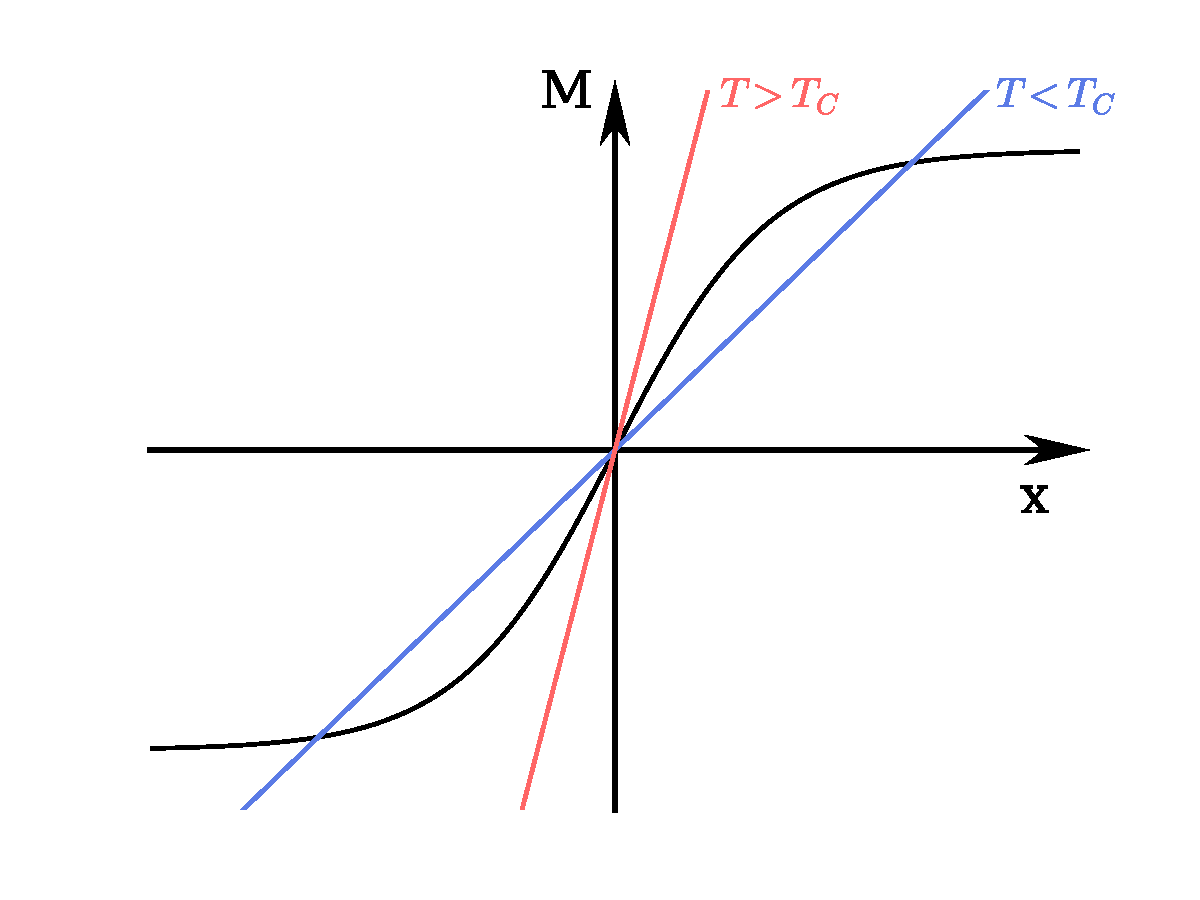
\includegraphics[width=0.916\linewidth]{../img/ferromag_graph_sol.pdf}
%   \captionsetup{width=6.9cm}
    \captionsetup{width=.95\linewidth}
    \captionof{figure}{Illustration of the grafical solution of \ref{eq:ferromag_graph_sol}. the straight lines refer to different values of of $T$.}
  \end{minipage}%
  \begin{minipage}[c][6.00cm]{.5\textwidth}
    \vspace*{\fill}
    \centering
    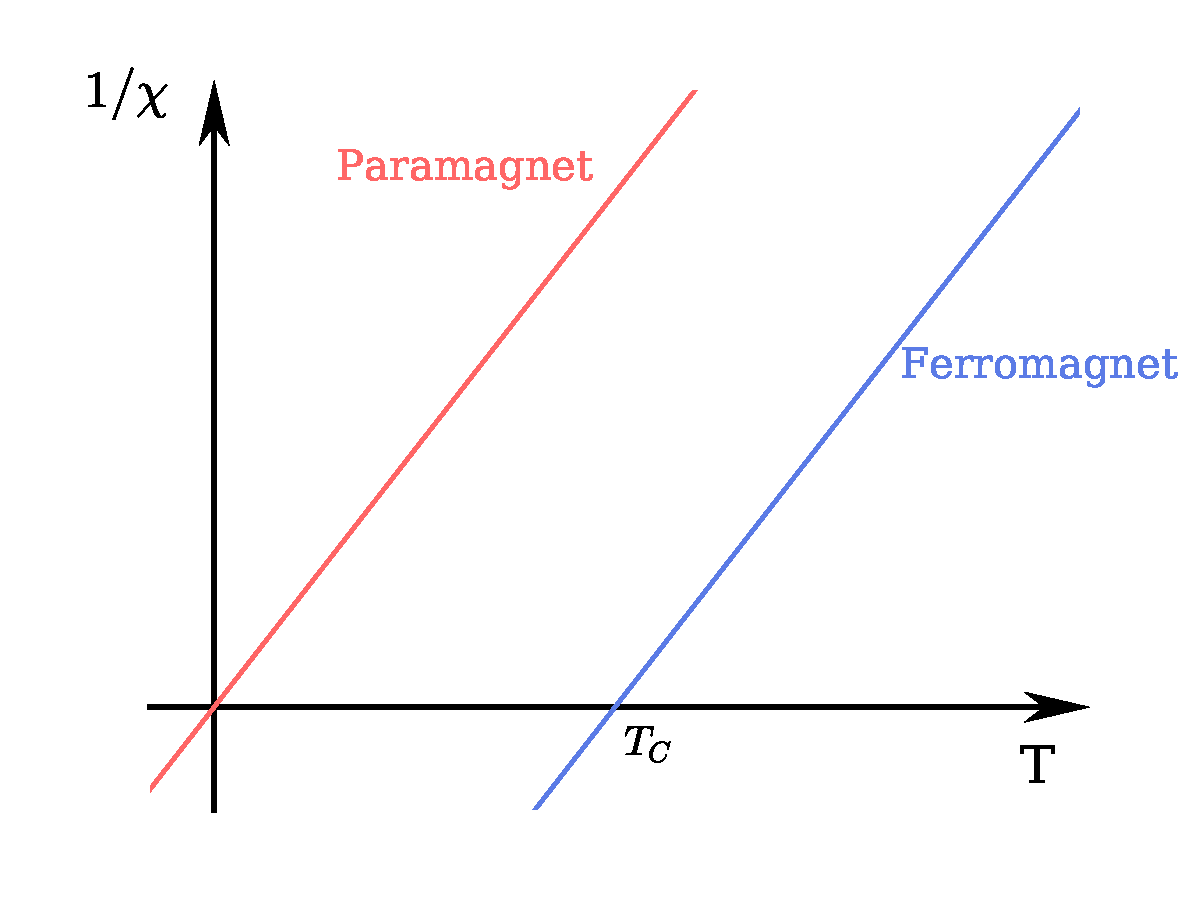
\includegraphics[width=0.95\linewidth]{../img/ferro_para_compar.pdf}
    \captionsetup{width=.95\linewidth}
 %   \captionsetup{width=6.9cm}
    \captionof{figure}{Illustration of susceptibility $\chi$ of a Para- and Ferromagnet.}
  \end{minipage}
  \label{fig:2:tests}
\end{figure}


%\begin{figure}
%  \centering
%  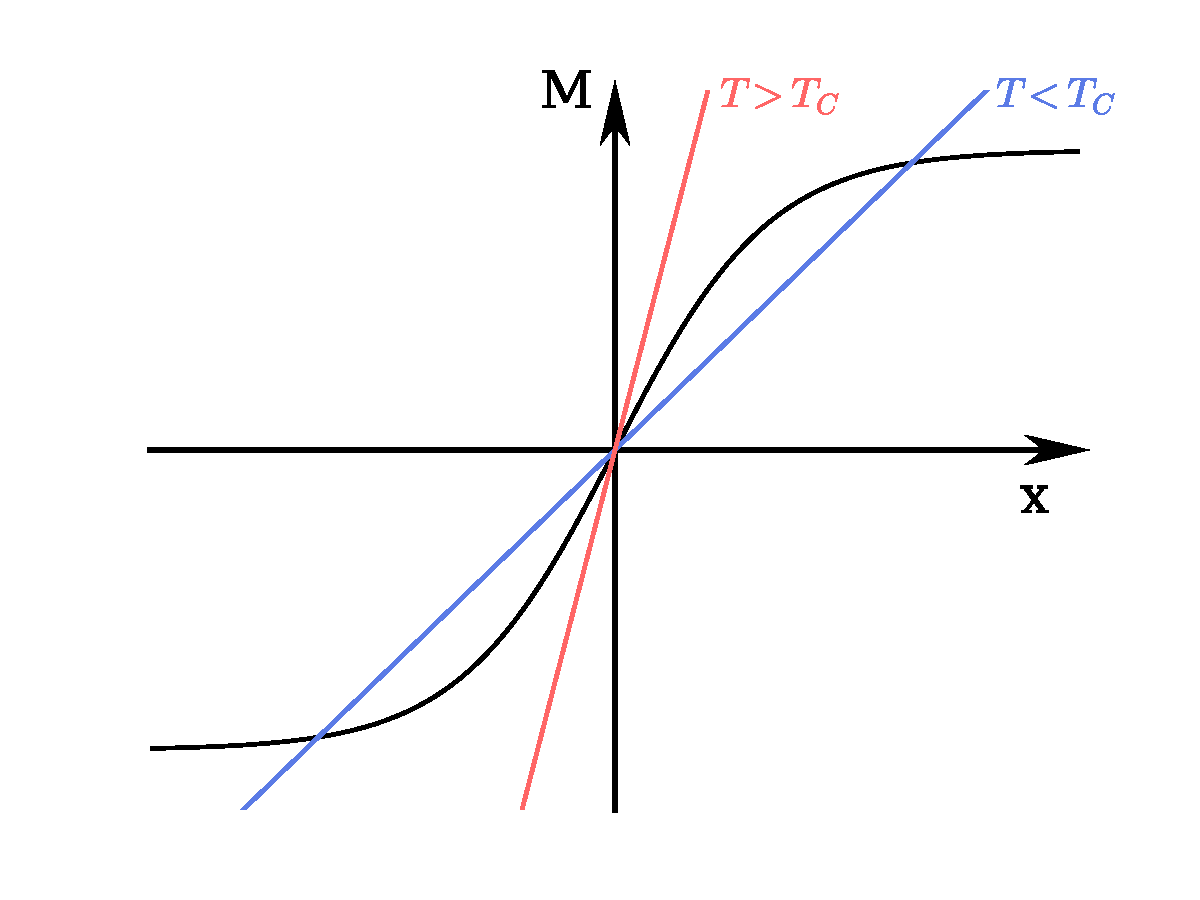
\includegraphics[width=0.5\linewidth]{../img/ferromag_graph_sol.pdf}
%  \caption{Illustration of the grafical solution of \ref{eq:ferromag_graph_sol}. the straight lines refer to different values of of $T$.}
%  \label{fig:ferromag_graph_sol}
%\end{figure}




Looking at the limit $ x \ll 1$ 

\begin{equation*}
  \left.
  \begin{array}{lcr}
    M ~ & = &~ C B/T \\
    \chi ~ & \equiv &~ M/B ~=~ C/T
  \end{array} \right\} 
  ~~~~ \rightarrow ~~~~ 
  \begin{array}{lcr}
    M ~~&=& ~ C \frac{B + \lambda M}{T}\\
    \chi ~ &\equiv& ~ \frac{C}{T} + \frac{\lambda}{T} \chi
  \end{array}
  ~~~~ \Rightarrow ~~~~ 
  \chi ~=~ \frac{C}{T-\lambda C} ~=~ \frac{C}{T - T_C}
\end{equation*}


Checking the magnetisation $M(T)$ at zero field $\vec{B} = 0$. Using \ref{eq:ferromag_graph_sol} with zero field and the definitinos $m = M/N \mu_B$ and $t = k_BT/N \mu_B^2 \lambda = T/T_C$ we get

\begin{equation}
  m ~~=~~ \tanh(\frac{m}{t})
\end{equation}

\begin{figure}[t]
  \begin{minipage}[c][6.00cm]{.5\textwidth}
    \vspace*{\fill}
    \centering
    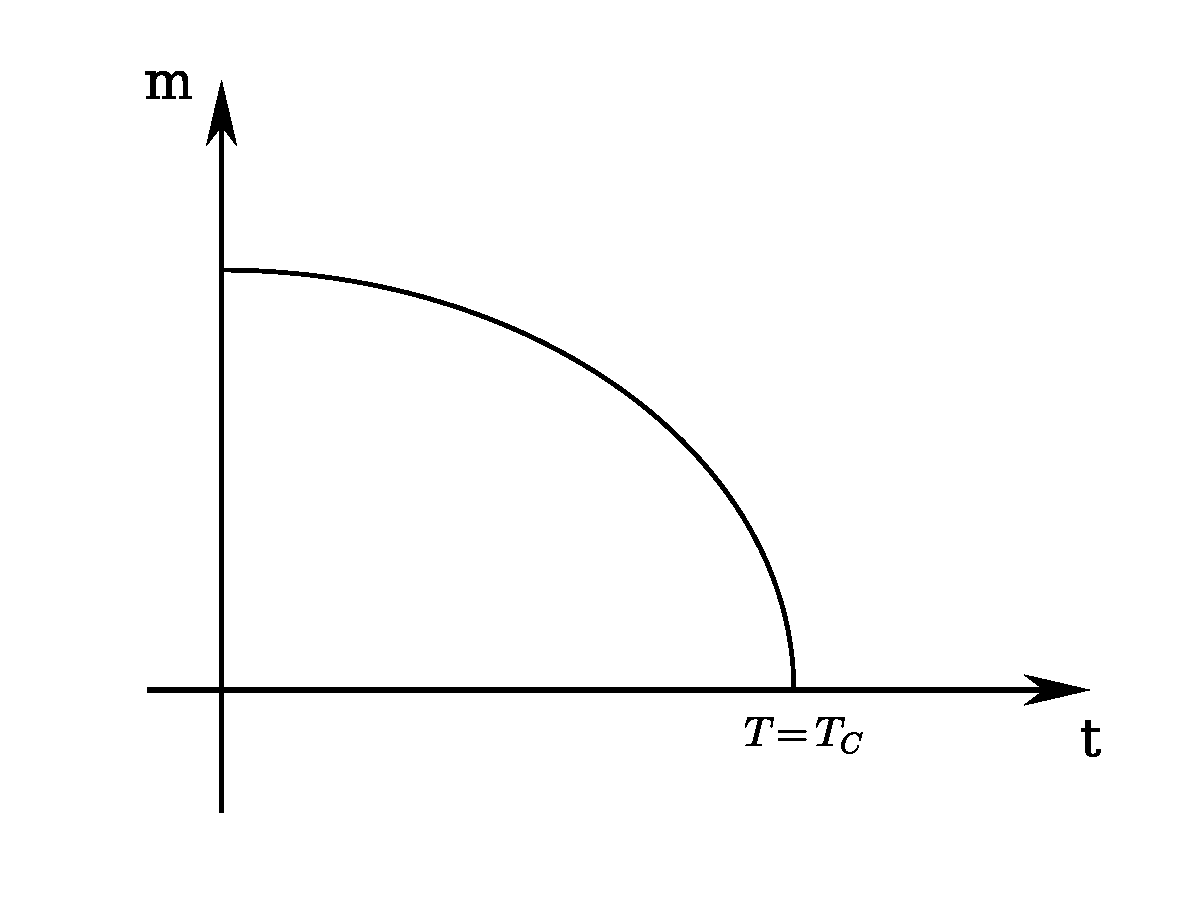
\includegraphics[width=0.916\linewidth]{../img/ferromag_M_T.pdf}
%   \captionsetup{width=6.9cm}
    \captionsetup{width=.95\linewidth}
    \captionof{figure}{Temperature dependence of magnetisation.}
  \end{minipage}%
  \begin{minipage}[c][6.00cm]{.5\textwidth}
    \vspace*{\fill}
    \centering
    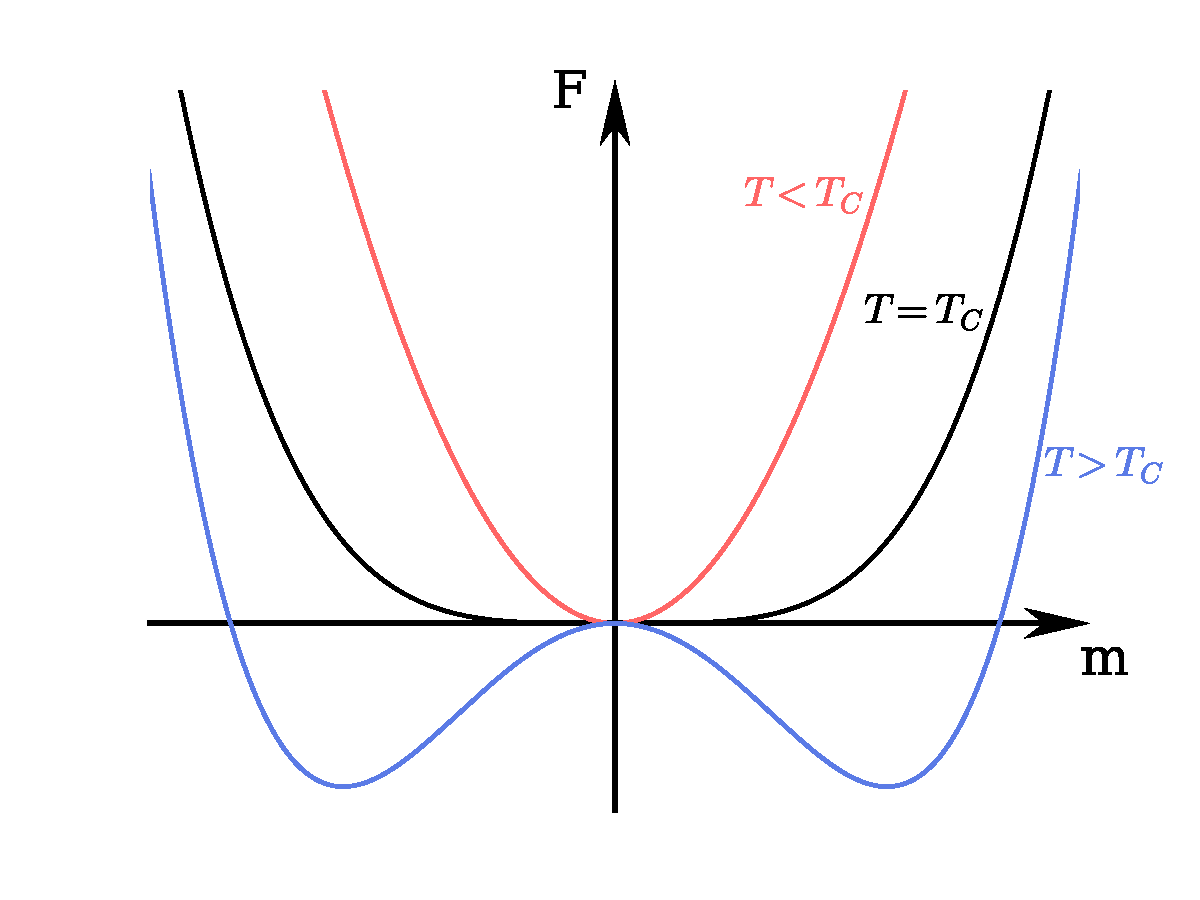
\includegraphics[width=0.95\linewidth]{../img/ferromag_landau.pdf}
    \captionsetup{width=.95\linewidth}
 %   \captionsetup{width=6.9cm}
    \captionof{figure}{Free Energy dependence on the order parameter $m$ for the 3 cases $T<T_C$, $T=T_C$ and $T>T_C$.}
  \end{minipage}
  \label{fig:2:tests}
\end{figure}


\subsubsection{Landau Theory}

According to the Landau theory of phase transisiton the free energy $F$ can be expressed

\begin{equation} \label{eq:ferromag_landau}
  F ~~=~~ F_0 ~+~ a(T) m^2 ~+~ b m^4 + ... 
\end{equation}

Were the parameter $a$ and $b$ has to meet the conditions

\begin{equation} \label{eq:ferromag_landau_condition}
  a(T) ~=~ a_0(T-T_C) ~~~~ \text{and} ~~~~ b>0
\end{equation}

We find the thermodynamical state of our system by minimizing the free energy

\begin{equation}
  \frac{dF}{dm} ~=~ m ( 2a(T) ~+~ 4bm^2) ~=~ 0 ~~~~ \Rightarrow ~~~~ m ~=~ \left\{ 
  \begin{array}{c}
    0\\
    \pm \sqrt{\frac{a_0(T-T_C)}{2b}}
  \end{array}
  \right.
\end{equation}



\subsection{Exchange Interaction J}


\begin{figure}
  \centering
  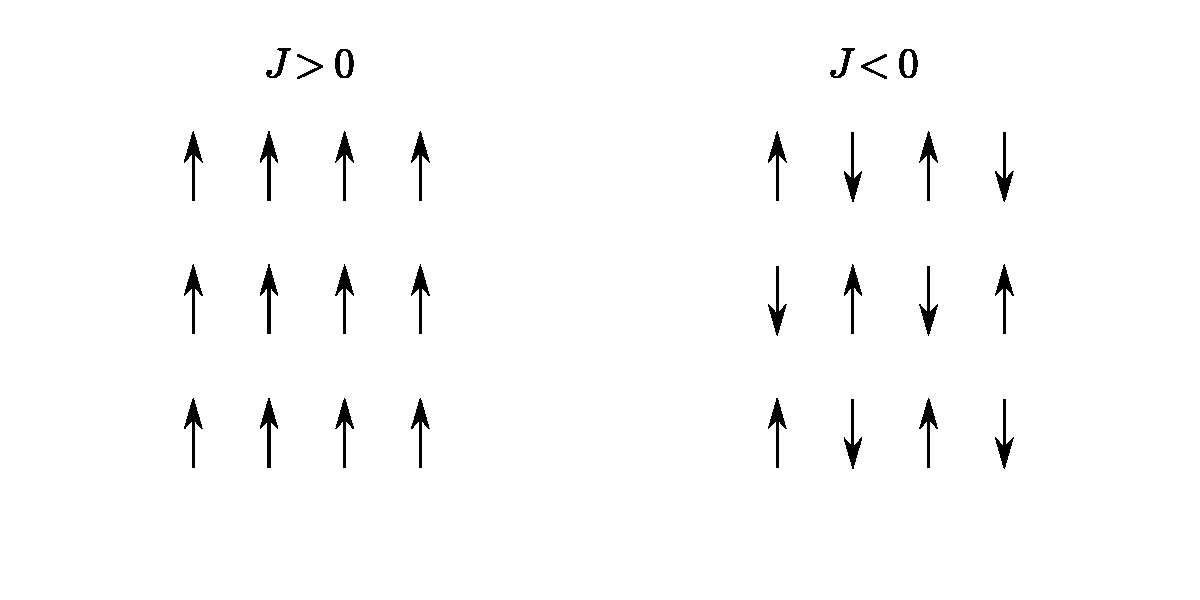
\includegraphics[width=0.7\linewidth]{../img/exch_spin_config.pdf}
  \caption{hohoho}
\end{figure}


Analog to the susceptibility of ferromagnets $\chi_{FM} = C/(T-T_C)$, we can define the susceptibility for anti-ferromagnets

\begin{equation}
  \chi_{AFM} ~~=~~ \frac{C}{T+T_N}
\end{equation}

Where we refer to the Transition Temperature $T_N$ as Neel-Temperature.


\begin{figure}[t]
  \begin{minipage}[c][6.00cm]{.5\textwidth}
    \vspace*{\fill}
    \centering
    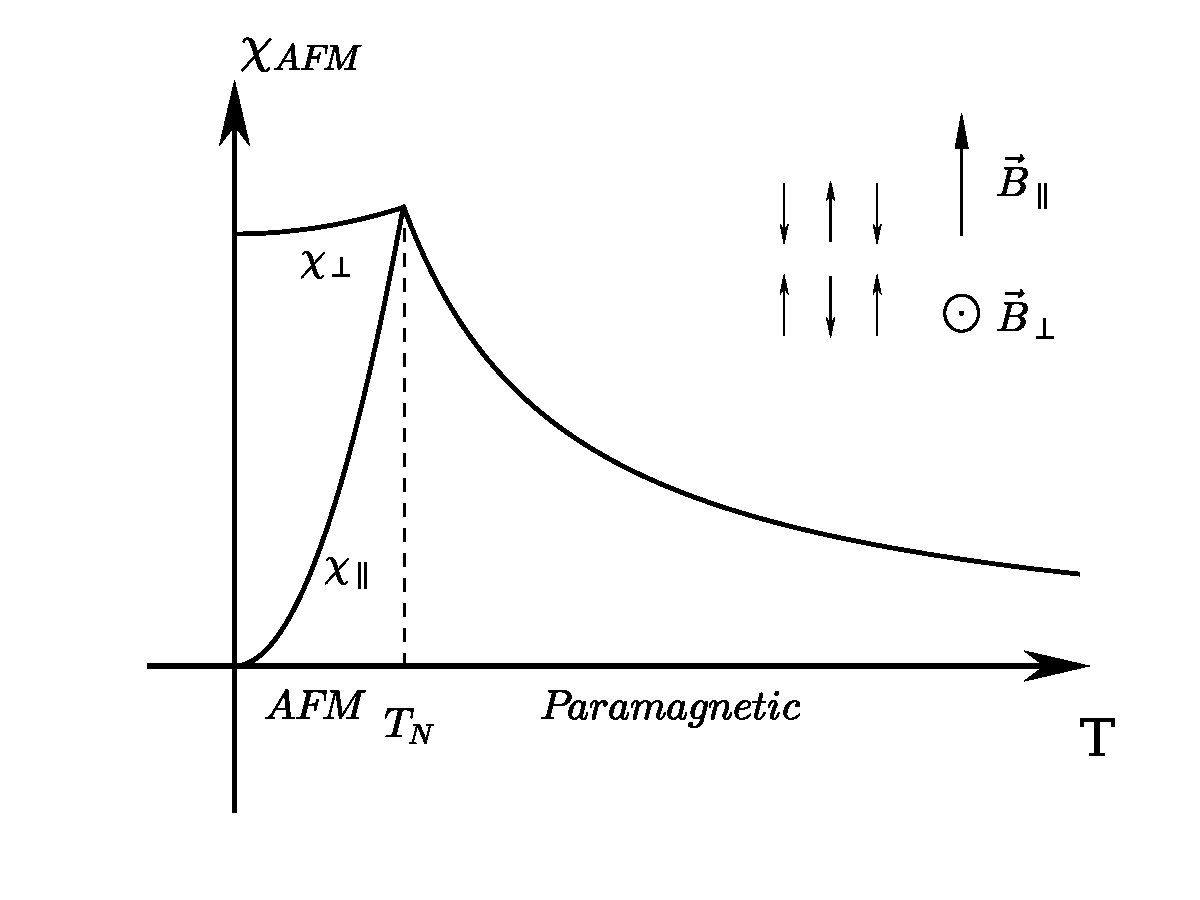
\includegraphics[width=0.916\linewidth]{../img/antiferro_suscept.pdf}
%   \captionsetup{width=6.9cm}
    \captionsetup{width=.95\linewidth}
    \captionof{figure}{Temperature dependence of magnetisation.}
  \end{minipage}%
  \begin{minipage}[c][6.00cm]{.5\textwidth}
    \vspace*{\fill}
    \centering
    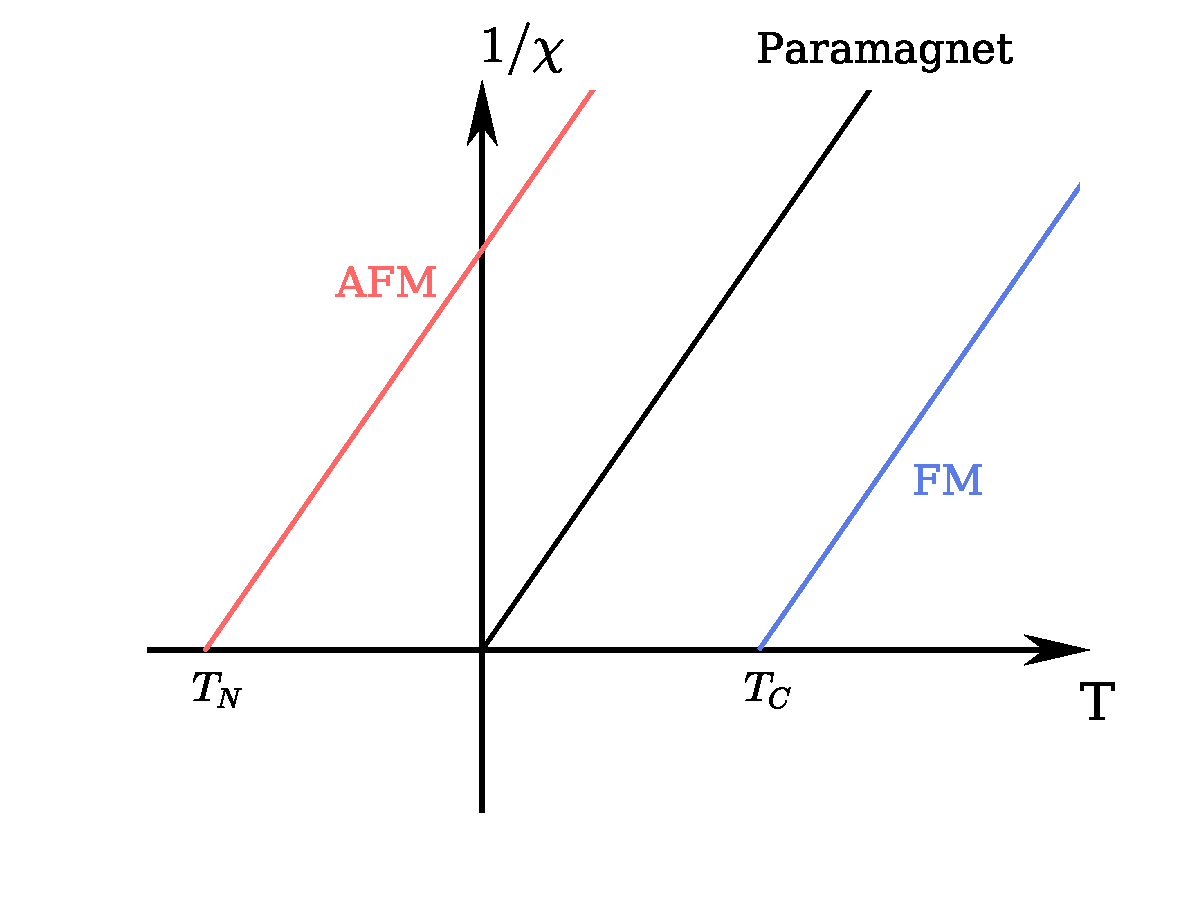
\includegraphics[width=1.0\linewidth]{../img/antiferro_para_compar.pdf}
    \captionsetup{width=1.0\linewidth}
 %   \captionsetup{width=6.9cm}
    \captionof{figure}{Free Energy dependence on the order parameter $m$ for the 3 cases $T<T_C$, $T=T_C$ and $T>T_C$.}
  \end{minipage}
  \label{fig:2:tests}
\end{figure}


\subsection{Ferromagnetic Magnons}

Consider a linear FM chain $ | \text{FM} \rangle ~=~ | \uparrow~ \uparrow~ \uparrow~ ...~ \rangle$. Applying the latter operator $ s^-_j$ onto this expression leads to

\begin{equation}
  | j \rangle ~~=~~ s^-_j | \text{FM} \rangle ~~=~~ 
  | \uparrow~ \uparrow~ ...~ \uparrow \underbrace{\downarrow}_{j} \uparrow~ ...~ \rangle
\end{equation}


Defining

\begin{equation}
  | q \rangle ~~=~~ \frac{1}{\sqrt{N}} \sum_j e^{i q R_j} | j \rangle
\end{equation}

The Hamilton is given as 

\begin{align}
  H ~~& =~~ - \sum_{ij} J_{ij} \hat{S}_i \cdot \hat{S}_j ~~=~~ -2J \sum_i \hat{S}_i \cdot \hat{S}_{i+1}\nonumber \\
      & =~~ - 2J \sum_i \left\{ \hat{S}^z_i \hat{S}^z_{i+1} ~+~ 
      \frac{1}{2} \left[ \hat{S}^+_i \hat{S}^-_{i+1} + \hat{S}^-_i \hat{S}^+_{i+1} \right]  \right\}
\end{align}

By taking only nearest neighbour interactions into account we get the 
The second equality sign holds if we only take neares neighbour interactions into account. To get the final expression we used the substitution

\begin{equation}
  \hat{S}^2 ~~=~~ \hat{S}^{z^2} ~+~ \frac{1}{2} \left[ \hat{S}^+_i \hat{S}^-_{i+1} + \hat{S}^-_i \hat{S}^+_{i+1} \right]
\end{equation}


\begin{equation}
  H | \text{FM} \rangle ~~=~~ -2 J N S^2 | \text{FM} \rangle ~~=~~ E_0 | \text{FM} \rangle
\end{equation}

\begin{equation}
  H | j \rangle ~~=~~ -2J \left\{ (N-4) S^2 | j \rangle ~+~ S \left[ |j+1\rangle + |j-1\rangle \right] \right\}
\end{equation}

\begin{align}
  H | q \rangle ~~& =~~ \frac{1}{\sqrt{N}} \sum_j e^{i q R_j} \left\{
  NS^2 |j\rangle ~-~ 2S^2|j\rangle ~+~ S |j+1\rangle ~+~ S|j-1\rangle \right\} \nonumber \\
                  & =~~ -2JNS^2 |q\rangle - 2J \left\{ -2S^2 ~+~ \left( e^{iqa} + e^{-iqa} \right) \right\} |q\rangle \nonumber \\
                  & =~~ E_0 |q\rangle ~+~ 2JS \left\{ 1 - \cos(qa) \right\} |q\rangle 
\end{align}

%%%% one equation not transcripted from lecture notes %%%


Since we are consindering an infinit long 1D chain of spin states we can rewrite the expression

\begin{equation}
  H |q\rangle ~~=~~ E_0 |q\rangle + 2JS \left\{ 2 - 2\cos(qa) \right\} |q\rangle
\end{equation} 

which leads to

\begin{equation}
  H |q\rangle ~~=~~ E(q) |q\rangle ~~~~~ \text{with} ~~~~ E(q) ~≃~ E_0 + 2JS(2 - 2\cos(qa))
\end{equation}

This is the dispersion relation for ferromagnets. For anti-ferromagnets we have a similar relation (not derived)

\begin{equation}
  \hbar \omega ~~=~~ 2J | \sin(qa) |
\end{equation}


%===============================================================================================================
% Superconductivity
%===============================================================================================================

\chapter{Superconductivity}

\section{Conventional superconducters}

\subsection{Link $\rho$ \& Meissner Effect}

\begin{figure}
  \centering
  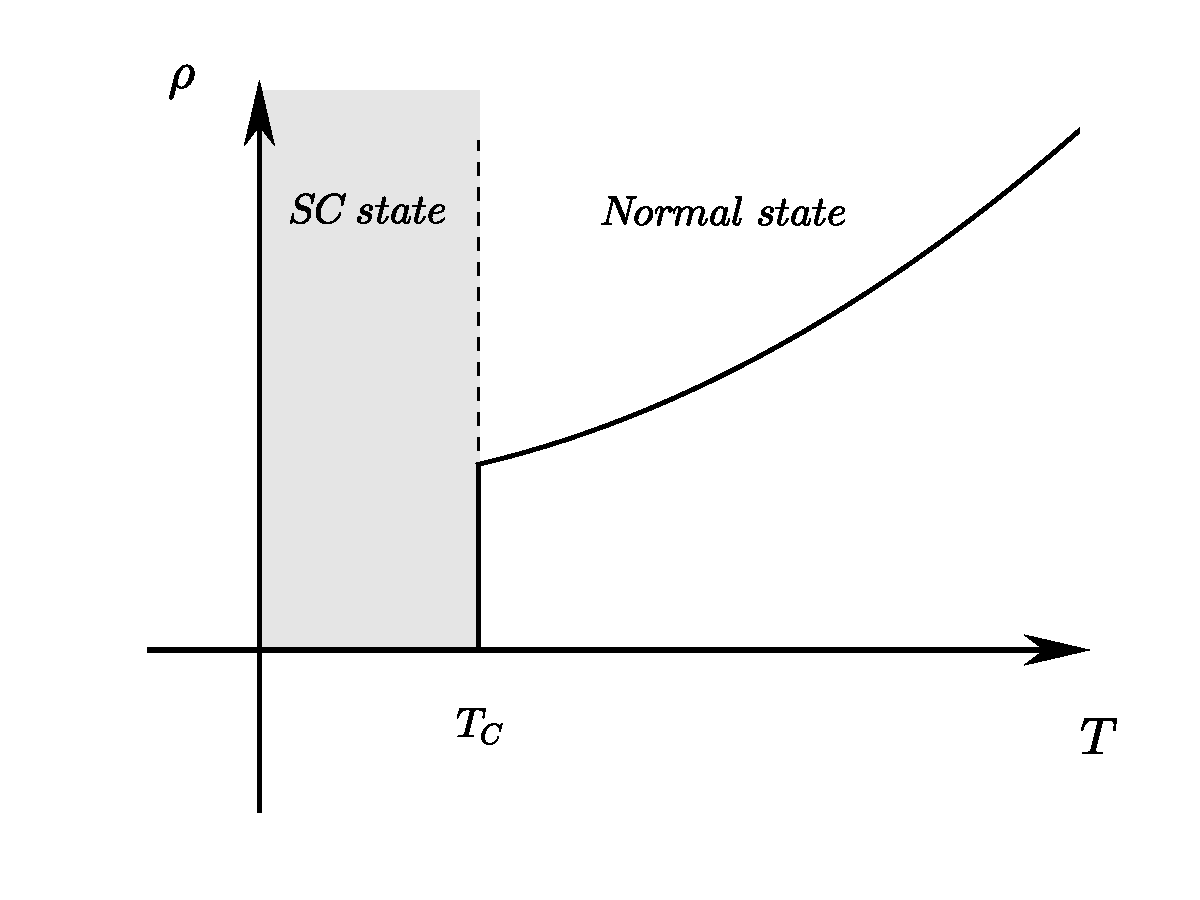
\includegraphics[width=0.7\linewidth]{../img/sc_resistivity_drop.pdf}
  \caption{hohoho}
  \label{fig:sc_res_drop}
\end{figure}


As we know, superconductors are characterised by vanishing resistvity ($\rho=0$) for undergoing a critical temperature $T_C$ (\myRef{fig:sc_res_drop}).
Recalling Ohm's law, 

\begin{equation} \label{eq:ohms_law}
  \vec{j} ~~=~~ \sigma \vec{E}
\end{equation}


which relates the electron current density $\vec{j}$ and the electric field inside a conductor $\vec{E}$ by introductin the material dependent conductivity $\sigma$.

Looking at the case of superconductors, we can emphasize, by rearranging Ohm's law, that the electric field vanishes.

\begin{equation}
  \vec{E} ~~=~~ \frac{1}{\sigma} \vec{j} ~~=~~ \rho \vec{j} ~~≃~~ 0
\end{equation}

By using one of the Maxwell equation $\nabla \times \vec{E} = - d\vec{B}/ dt$ we can conclude, that for a vanishing electric field $\vec{E} = 0$ there can't be a change of the magnetic field over time $d\vec{B}/dt=0$.


\textcolor{red}{diagram vanishing B-field}


\section{London Equation}

The lonodon equation is a macroscopic theory that was one of the first theories which allowed to describe effects like the Meissner-Ochsenfeld effect quantitatively.
We know want to qualitiatively derive the london equation. For that consider a current oscillating if the frequency $\omega$

\begin{equation}\label{eq:osc_curr}
  \vec{j} e^{-i \omega t} ~~=~~ \sigma(\omega) \vec{E} e^{-i \omega t}
\end{equation}

Using the expression for the conductivity $\sigma(\omega)$ from the Drude model for a time-dependent electric field

\begin{equation}
  \sigma(\omega) ~~=~~ \frac{\vec{j}}{\vec{E}} ~~=~~ \frac{ne^2 \tau}{m} \frac{1}{1-i\omega \tau}
\end{equation}

%Looking at the real part of the conductivity
%
%\begin{equation}
%  \Re(\sigma(\omega)) ~~=~~ \frac{ne^2}{m} \frac{\tau}{1+\omega \tau}~~ \xrightarrow{\omega \rightarrow 0} ~~
%  \frac{ne^2 \tau}{m}
%\end{equation}

From this we get, as already proven in a previous excercise, that the real part of the conductivity can be written in the limit of $\tau \rightarrow \infty$ as

\begin{equation}\label{eq:real_conduct}
  \Re(\sigma(\omega)) ~~=~~ \frac{\pi n e^2}{m} \delta(\omega)
\end{equation}


This can also be made clear, when looking at the limits

\begin{equation}
  \Re(\sigma(\omega)) ~~=~~ \frac{ne^2}{m} \frac{\tau}{1+\omega \tau}~~ \xrightarrow{\omega \rightarrow 0} ~~
  \frac{ne^2 \tau}{m}
\end{equation}

\begin{equation}
  \sigma(\omega) ~~ \xrightarrow{\tau \rightarrow \infty} ~~ -\frac{ne^2}{im\omega} = \Im(\sigma(\omega)) ~~~~ \Rightarrow ~~~~ \Re(\sigma(\omega)) = 0 ~~~~~~\text{for}\ \omega \neq 0
\end{equation}


From \myEq{eq:real_conduct}, we see that in the regime of very large mean free times $\tau$ between ionic collisions, the real part of the conductivity $\sigma(\omega)$ is only different from zero for vanishing oscillations of the electric field. 

To derive the London equation, the following two assumptions have to be made

\begin{enumerate}
\item{$\tau \rightarrow \infty$, which is given since there are no collisions between electrons and lattice ions in the superconducting state.}
\item{We have to split up the conductivity in a part $\sigma_{N}(\omega)$ of normal state electrons and a conductivity contribution due to \textit{super electrons} $\sigma_{S}$: 
$\sigma(\omega) = \sigma_N(\omega) + \sigma_S(\omega)$, were only $\sigma_S(\omega) \neq 0$ in the superconducting state}
\end{enumerate}


Taking the curl of the oscillating current

\begin{align}\label{eq:curl_curr}
  \nabla \times (\vec{j} e^{-i\omega t}) & ~~=~~ -\sigma(\omega) \nabla \times (\vec{E}\cdot e^{-i\omega t}) ~~=~~
  -\sigma(\omega) \frac{d}{dt} (\vec{B} \cdot e^{-i\omega t})\nonumber \\
    & ~~=~~ - \frac{n_Se^2}{m} \vec{B} \cdot e^{-i\omega t}
\end{align}

Here we used \myEq{eq:osc_curr} in the first and farradays law ($\nabla \times \vec{E} = d/dt \vec{B}$) in the second step. Furthermore is only the \textit{super electron} density $n_S$ contributing to the conductivity $\sigma(\omega)$. From this equation we can deduce that

\begin{equation}\label{eq:london_eq}
  \nabla \times \vec{j} ~~\propto~~ \vec{B} ~~~~~~\text{and thereof}~~~~ \vec{j} = -\frac{n_Se^2}{m} \vec{A}
\end{equation}

with $\vec{A}$ being the vector potential. The equation describing this proprtionality between the current density $\vec{j}$ and the vector potential $\vec{A}$ is the London equation.


%The london equation allows us now to set up a differential equation for the magnetic field $\vec{B}$. 
%
Together with Ampere's law ($\nabla \times \vec{B} = \mu_0 \vec{j}$) allows us the London equation (\myEq{eq:london_eq}) now to set up a differential equation for the magentic field $\vec{B}$.

\begin{equation} \label{eq:deq_B_0}
  \nabla \times \nabla \times \vec{B} ~~=~~ -\frac{1}{\lambda^2} \vec{B}, ~~~~~~ \text{where}~~ 
  \lambda = \sqrt{\frac{m}{\mu_0 n_S e^2}}
\end{equation}

This equation can also be written as

\begin{equation} \label{eq:deq_B}
  \nabla^2 \cdot \vec{B} ~~=~~ \frac{1}{\lambda^2} \vec{B}
\end{equation}


To exemplify the solution of this differential equation we look at it in one dimension. Then \myEq{eq:deq_B} becomes $d^2/dx^2 B_z(x) = 1/\lambda^2 B_x$.

To exemplify the solution of this differential equation we look at a situation were we have a superconductor filling the space for all values $x\geq 0$ correspinding to that we have vacuum at $x<0$. Applyling now a magnetic field in the vacuum region aligned along the z-axis $\vec{B} = (0,0,B_0)$. in this case the differential equation \myEq{eq:deq_B} simplifies to 

\begin{equation}
  \frac{d^2}{dx^2} B_z(x) ~~=~~ \frac{1}{\lambda^2} B_z(x)
\end{equation}

Using the boundary conditions $B_z(x) \xrightarrow{x \rightarrow \infty} 0$ (Meissner Effect) and $B_z(x \rightarrow 0)=B_0$ leads to the solution

\begin{equation} \label{eq:B_decrease}
  B_z(x) ~~=~~ B_0 e^{-x/\lambda}
\end{equation}

This solution describes an exponentially decreasing magnetic field inside the the superconductor close to the surface. From this formula one can also recognize that $\lambda = \sqrt{m/\mu_0 n_S e^2}$ introduced a characteristic length scale over which the magnetic penetrates the superconductor. For that reason $\lambda$ is referred to as \textit{London penetration depth}. 
In \ref{fig:london_lambda} we see \myEq{eq:B_decrease} plotted for two different values of lambda $\lambda_1 > \lambda_2$. 
Looking at the definition of the London penetration depth we see that $n_{S_1} < n_{S_2}$, which means that the higher the charge density the more is the penetrating magnetic field $B_z(x)$ diminished.


\begin{figure}[t]
  \begin{minipage}[c][6.00cm]{.5\textwidth}
    \vspace*{\fill}
    \centering
    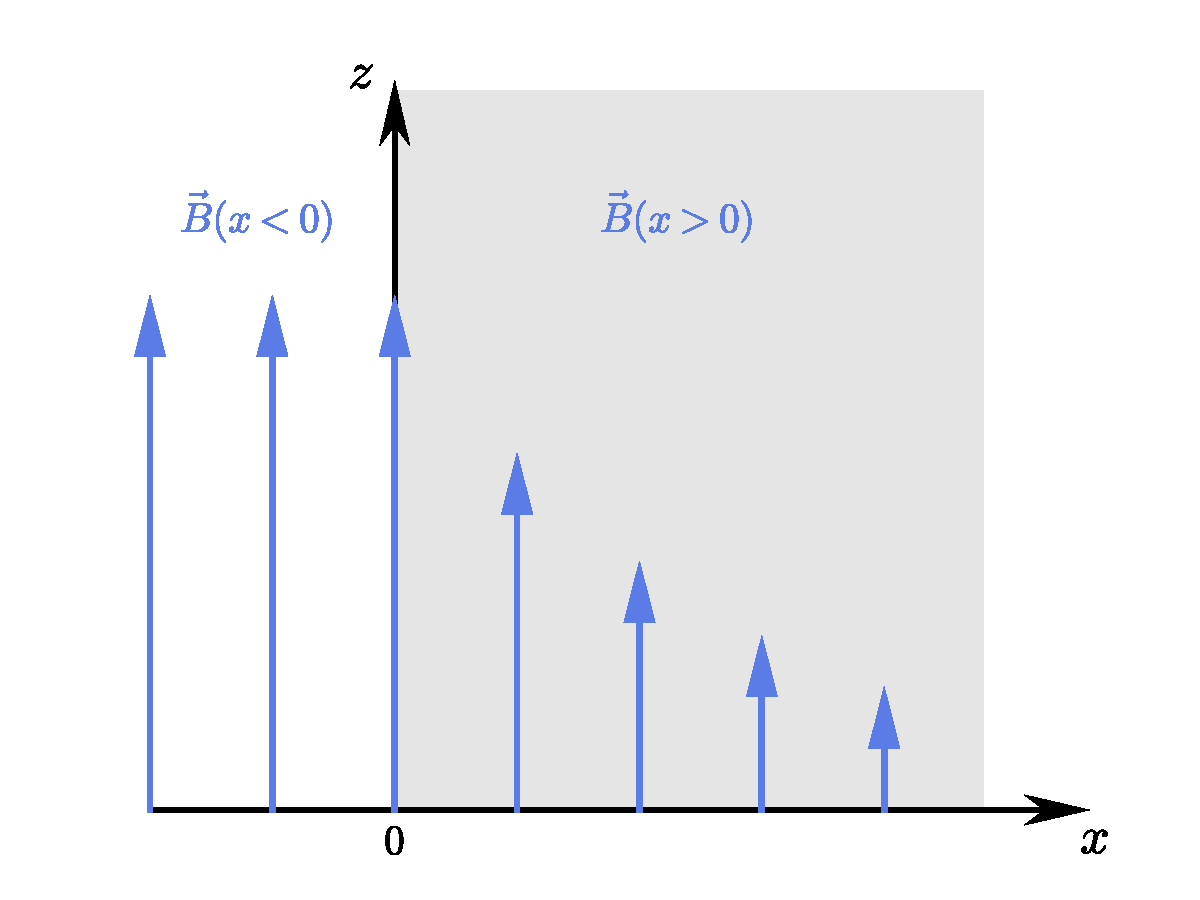
\includegraphics[width=0.916\linewidth]{../img/london_B_1dim.pdf}
%   \captionsetup{width=6.9cm}
    \captionsetup{width=.95\linewidth}
    \captionof{figure}{Illustration of the magnetic field decrease inside the superconductor according to \myEq{eq:B_decrease}. The magnetic field is pictorially drawn as blue vectors. Adapted from \text{red}{Kittel - include citation}}
    \label{fig:london_B_1dim}
  \end{minipage}%
  \begin{minipage}[c][6.00cm]{.5\textwidth}
    \vspace*{\fill}
    \centering
    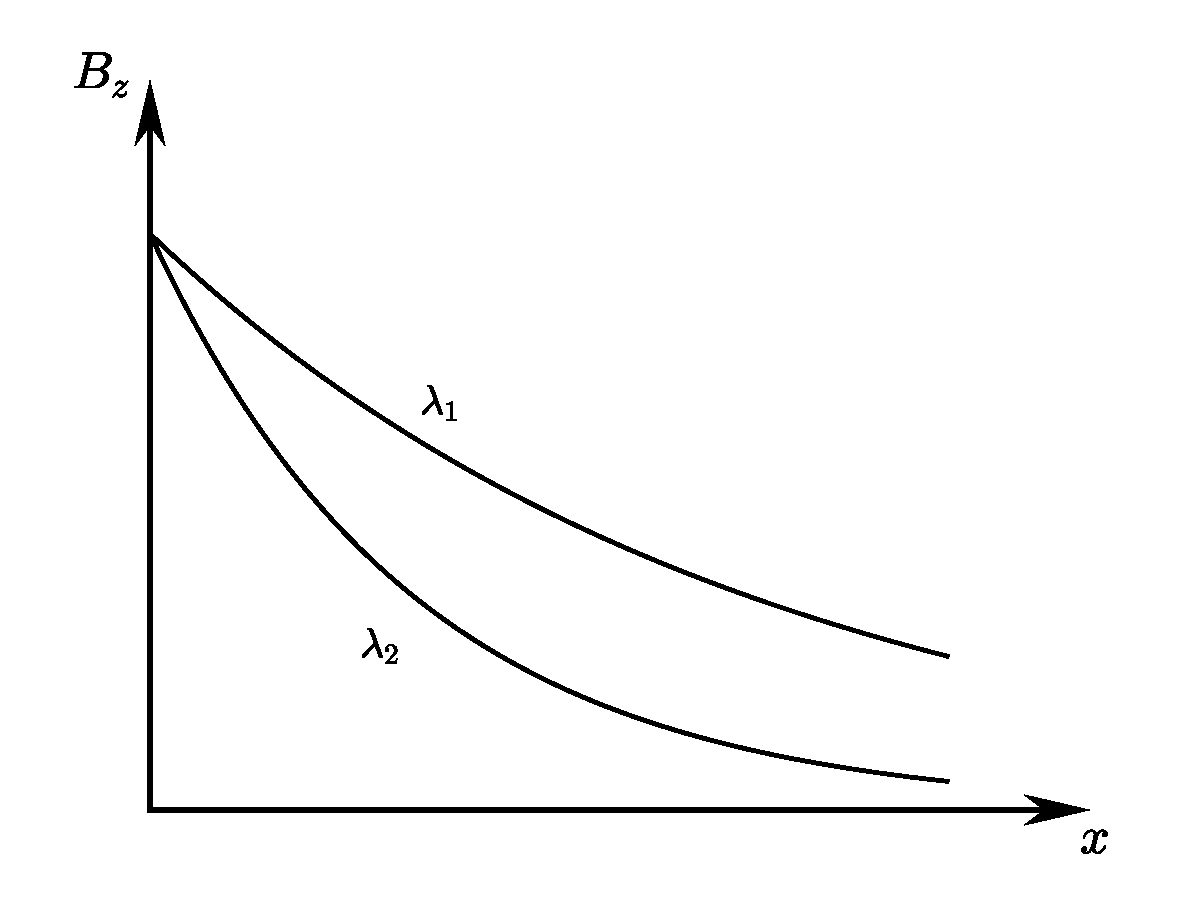
\includegraphics[width=1.0\linewidth]{../img/london_lambda.pdf}
    \captionsetup{width=0.95\linewidth}
 %   \captionsetup{width=6.9cm}
    \captionof{figure}{Illustration of \myEq{eq:B_decrease} for two different values for the london penetration depth.}
    \label{fig:london_lambda}
  \end{minipage}
\end{figure}




\section{Coherence Length}

Another lengthscale that helps us to classify the different types of superconductors is the \textit{coherence length} $\xi$. The coherence length is a measure of the distance within which the superconducting electron concentration cannot change drastically in a spatially-varying magnetic field.

\begin{equation} \label{eq:coherence_length}
  \xi ~~=~~ \frac{\hbar v_F}{\pi \Delta}
\end{equation}

Where $v_F$ stands for the fermi velocity and $\Delta$ for superconducting gap being present at the fermi surface in the SC state. $\xi$ is a parameter in the \textit{Ginzburg-Landau Theory} and can be derived there.

The two length scales, penetration depth and coherence length, allow us now, to categorize the superconductors in the groups \textit{Type 1} and \textit{Type 2}. This goes as follows:

By defining $\kappa \equiv \xi/\lambda$ we say a Superconductor contains to the group of \textit{Type 1} (\textit{Type 2}) if $\kappa ~<~ (>)~ 1/\sqrt{2} \simeq 0.707 $. 

Values of $\kappa$ for some materials are given in \textcolor{red}{lenght scale table}. The classification of SC into Type 1 and Type 2 does not fully coincide with the classification of conventional and unconvential. Although a lot of the conventional (elementary) supperconductors are of Type 1, there are also some expetions like Niobium (Nb) which is a conventional Type 2 Superconductor.

\textcolor{red}{include table from PPP}


\section{Ginzburg-Landau Theory}

The Landau Theory of Phase Transtition can also be used in the case of the transition from normal to superconducting state. The free energy per volume of the system in the superconducting state is given as

\begin{equation}
  f_\text{SC} ~~=~~ f_\text{NS} ~+~ a(T) |\psi(T)|^2 ~+~ \frac{1}{2} b(T) |\psi(T)|^4 ~+~ ...
\end{equation}

$|\psi|$ is treated as the order parameter. 
To find the temperature dependence of the free energy per volumne we make the following assumptions: near the transition temperature $T_C$ has $a$ to be linear in temperature ($a(T)=a_0(T-T_C) +...$) and $b$ given as $b(T)=b_0+...$ with $a_0, b_0$ being constant and larger than zero.

Looking for the extrema of $(f_\text{SC}-f_\text{NS})$

\begin{equation} \label{eq:f_SC_derived}
  \frac{d (f_\text{SC}-f_\text{NS})}{d|\psi|} ~~=~~ 2|\psi| \left\{a(T) ~+~ b(T)|\psi|^2  \right\} 
  ~~\overset{!}{=}~~ 0
\end{equation}

We find the following condition for $|\psi|$ to minimize $(f_\text{SC}-f_\text{NS})$

\begin{equation} \label{eq:psi_condition}
  |\psi| ~~=~~ \left\{ 
  \begin{array}{cr}
    0, & T>T_C\\
    \pm \sqrt{-a(T)/b(T)}, & T<T_C
  \end{array} \right.
\end{equation}

Plugging \myEq{eq:psi_condition} into \myEq{eq:f_SC_derived} leads to

\begin{equation}
  (f_\text{SC} - f_\text{NS}) ~~=~~ -\frac{a^2(T)}{b(T)} ~+~ \frac{1}{2} \frac{a^2(T)}{b(T)} ~~=~~
  -\frac{1}{2} \frac{a_0^2(T-T_C)^2}{b_0}
\end{equation}


\begin{figure}[t]
  \begin{minipage}[c][6.50cm]{.5\textwidth}
    \vspace*{\fill}
    \centering
    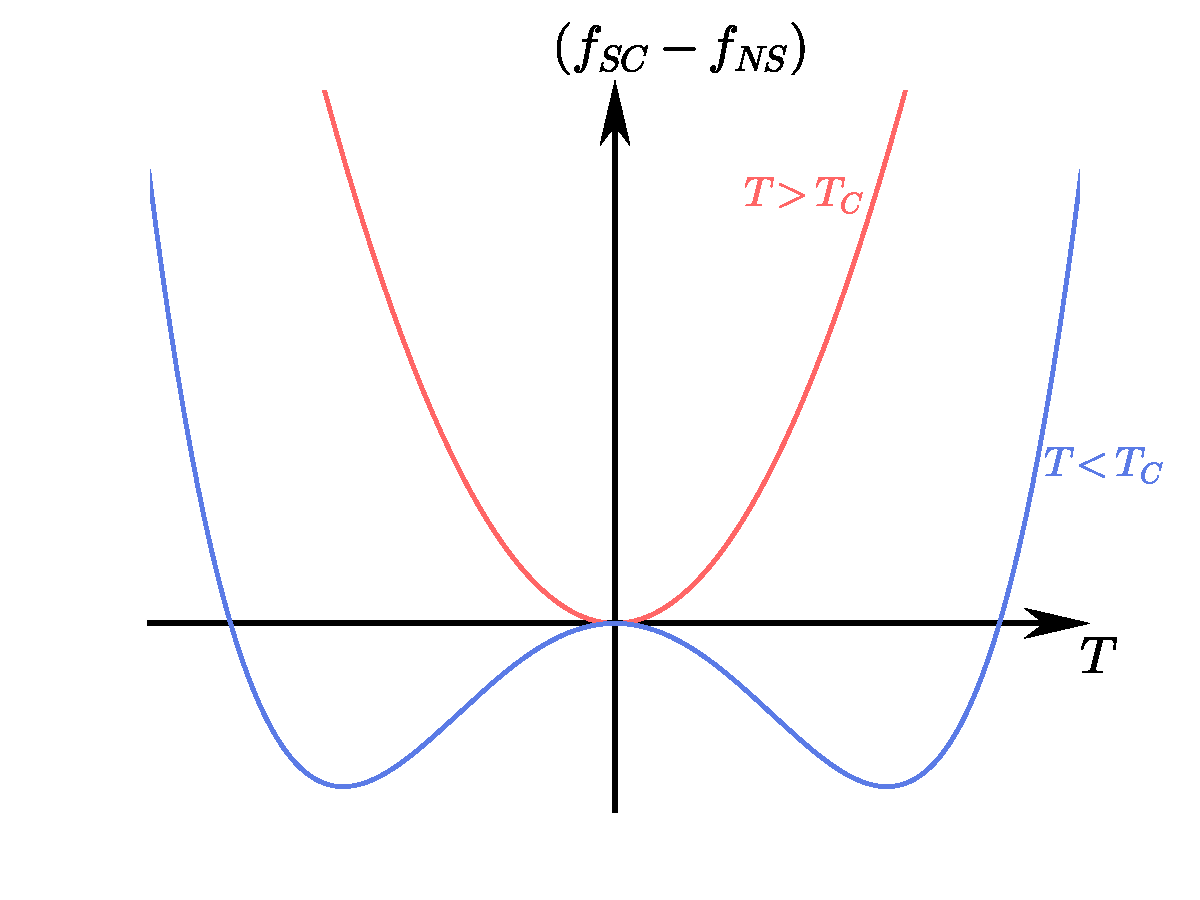
\includegraphics[width=0.916\linewidth]{../img/landauginzburg_f_SC.pdf}
%   \captionsetup{width=6.9cm}
    \captionsetup{width=.95\linewidth}
    \captionof{figure}{Difference of the free energy per volume between the normal- and superconducting state.}
    \label{fig:london_B_1dim}
  \end{minipage}%
  \begin{minipage}[c][6.00cm]{.5\textwidth}
    \vspace*{\fill}
    \centering
    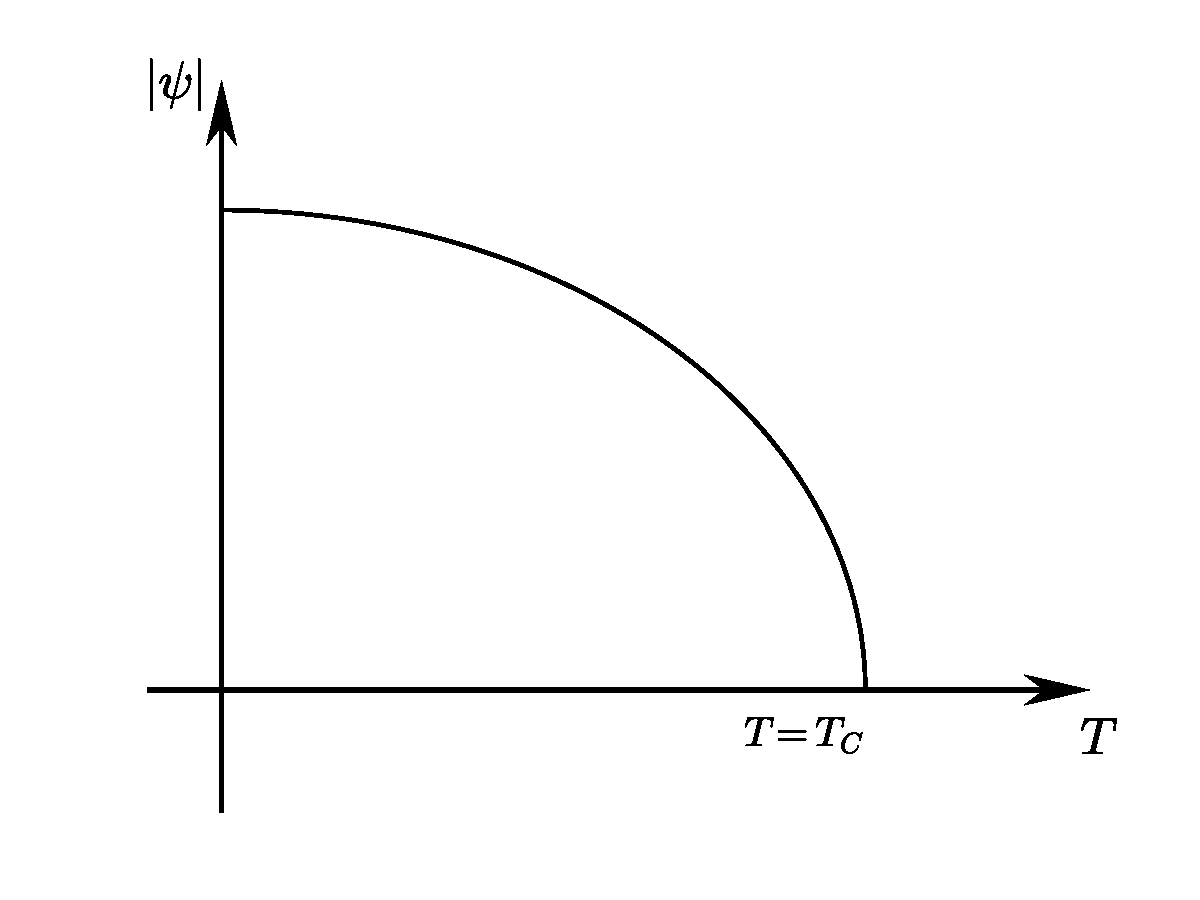
\includegraphics[width=1.0\linewidth]{../img/landauginzburg_psi_T.pdf}
    \captionsetup{width=0.95\linewidth}
 %   \captionsetup{width=6.9cm}
    \captionof{figure}{Temperature dependence of the order parameter $|\psi|$. }
    \label{fig:london_lambda}
  \end{minipage}
\end{figure}

Since $f_\text{SC}$ is the free energy, we can write

\begin{equation}
  S ~~\equiv~~ -\frac{df}{dT} ~~~~~~\text{and}~~~~~~ C ~~\equiv~~ T \cdot \frac{dS}{dT}
\end{equation}

This gives for the difference in the heat capacity

\begin{equation} \label{eq:diff_heat_cap}
  \Delta C ~~\equiv~~ C_\text{SC} ~-~ C_\text{NS} ~~=~~ -T \frac{d^2(f_\text{SC}-f_\text{NS})}{dT^2} 
  ~~=~~ T \frac{a_0^2}{b_0}
\end{equation}

Evaluating \myEq{eq:diff_heat_cap} at the transition Temperature gives us the jump in specific heat at the phase transition

\begin{equation}
  \Delta C(T_C) ~~=~~ \frac{a_0^2}{b_0} T_C
\end{equation}


\subsection{Orderparameter in the Ginzburg-Landau Model}

To point out the connection between the penetration depth resulting from the London Equation and the Ginzburg-Landau Theory, we look a bit closer at the order parameter $|\psi|$. Before we defined the term of the super electrons $n_s$ in the London's theory. In BCS-Theory this quantity is referred to as density of cooper pairs.

\begin{equation*}
  n_S ~~=~~ \left\{
  \begin{array}{lcr}
    \# \text{super electrons} & ~~\leftarrow~~ & \text{London Theory}\\
    \# \text{cooper pairs}    & ~~\leftarrow~~ & \text{BCS Theory}
  \end{array} \right.
\end{equation*} 


Here we assign 

\begin{equation}
  n_S ~~=~~ 2|\psi|^2 ~~=~~ 2 \frac{a_0(T_C-T)}{b_0}
\end{equation}

This allows us now to express the penetretion depth $\lambda$ from \myEq{eq:deq_B_0} as explicitly temperature dependent

\begin{equation} \label{eq:penetration_depth_temp_dep}
  \lambda(T) ~~=~~ \sqrt{\frac{b_0 m}{2 \mu_0 e^2 a_0 (T_C-T)}}
\end{equation}

\section{Classification of different superconductors}


\section{Vorteces}

To define the appearance of vorteces from Type 2 Superconductors into into our formalism we define the free energy per volumne as

\begin{equation} \label{eq:vortex_free_energy}
  f_\text{SC} - f_\text{NS} ~~≃~~ a(T) |\psi(r)|^2 ~+~ b(T)|\psi(r)|^4 ~+~ 
  \frac{\hbar^2}{2m} \nabla |\psi|^2
\end{equation}

To get the total Free energy we integrate \myEq{eq:vortex_free_energy} over all space

\begin{equation}
  F_\text{SC} - F_\text{NS} ~~=~~ \int d^3r (f_\text{SC} - f_\text{NS})
\end{equation}

We are interested now in finding the wavefunction $\psi(r)$ for which the Free energy is minimized. Since $\psi(r)$ is a function, this condition is formulated in a functional of the following form

\begin{equation}
  \frac{\delta F_\text{SC}}{\delta \psi(r)} ~~\overset{!}{=}~~ 0
\end{equation}

This is a differential equation for $\psi(r)$. In one dimnesion this DEG looks like the following

\begin{equation} \label{eq:vortex_wave_function_deg}
  -\frac{\hbar^2}{2m} \frac{d^2\psi(x)}{dx^2} ~+~ a(T) \psi(x) ~+~ b(T) \psi^3(x) ~~=~~ 0
\end{equation}

A solution to this differential equation is

\begin{equation} \label{eq:vortex_wave_function}
  \psi(x) ~~=~~ \psi_0 \tanh(\frac{x}{\sqrt{2} \xi(T)})
  \ 
\end{equation}


The coherence length $\xi(T)$ introduces a temperature dependent length scale and is given as

\begin{equation} \label{eq:vortex_coherence_length}
  \xi(T) ~~=~~ \left( \frac{\hbar}{2m |a(T)|} \right)^{1/2} ~~=~~ \xi_0\ t^{-1/2} ~~~~~~\text{with}~~~~ 
  t = \frac{T-T_C}{T_C}
\end{equation}

Here we used the same expression for $a(T)$ as in the ginzburg-Landau Theory.

\begin{figure}[t]
  \begin{minipage}[c][6.50cm]{.5\textwidth}
    \vspace*{\fill}
    \centering
    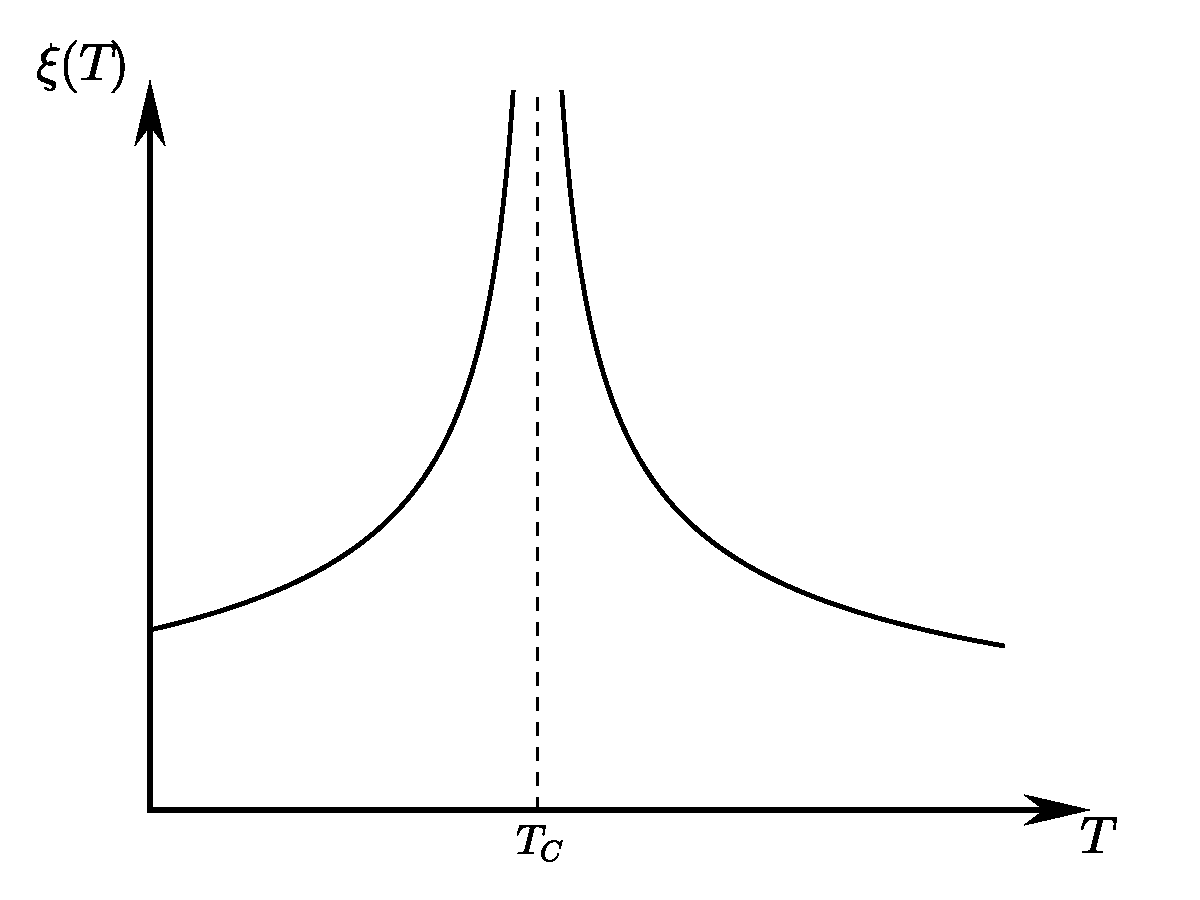
\includegraphics[width=0.916\linewidth]{../img/vortex_coherence_length.pdf}
%   \captionsetup{width=6.9cm}
    \captionsetup{width=.95\linewidth}
    \captionof{figure}{Coherence length $\xi(T)$ plotted over Temperature according to \myEq{eq:cortex_coherence_length}. Noteworthy is the diverging of $\xi$ when going close to $T_C$.}
    \label{fig:london_B_1dim}
  \end{minipage}%
  \begin{minipage}[c][6.00cm]{.5\textwidth}
    \vspace*{\fill}
    \centering
    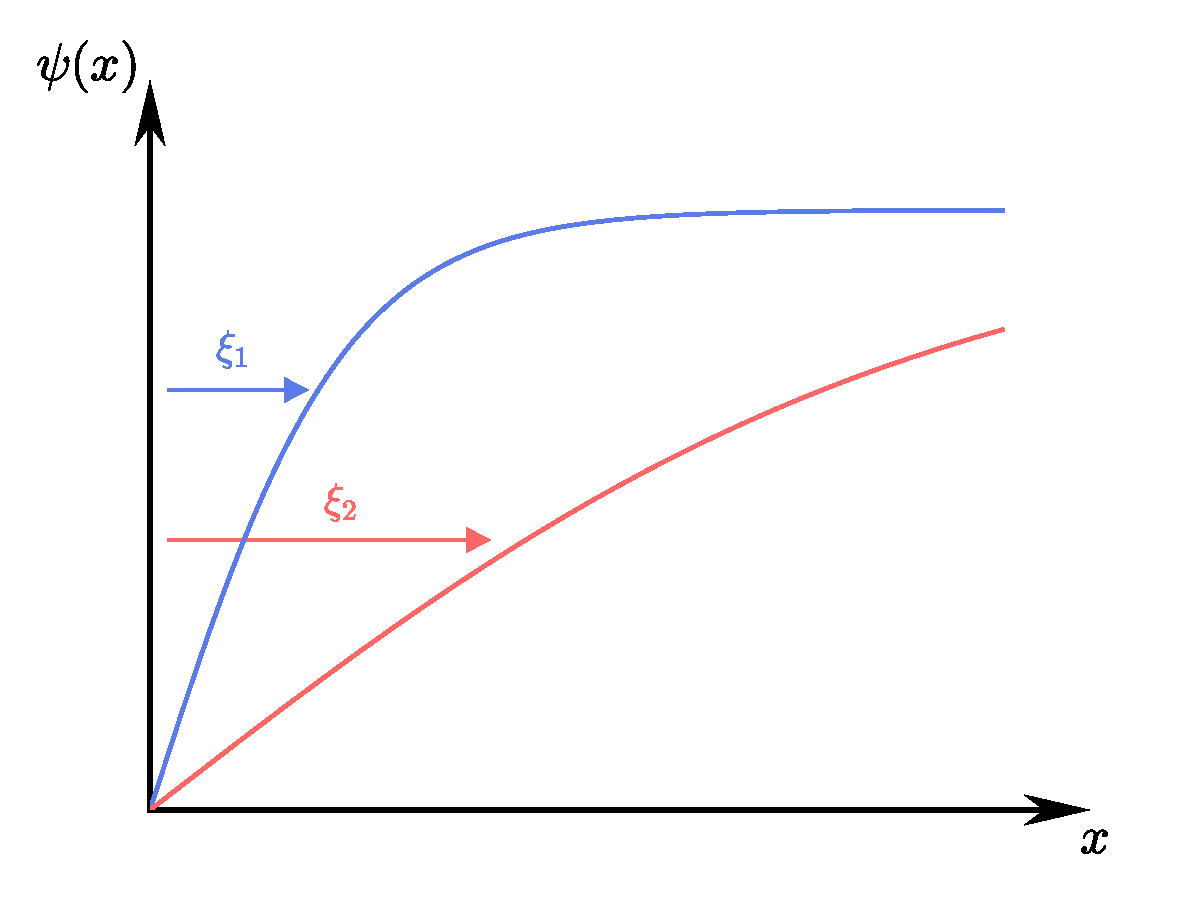
\includegraphics[width=1.0\linewidth]{../img/vortex_wavefunction.pdf}
    \captionsetup{width=0.95\linewidth}
 %   \captionsetup{width=6.9cm}
    \captionof{figure}{Wavefunction in one dimension according to \myEq{eq:vortex_wave_function}. Comparing the the blue and red curve shows that the wave function gets \textit{pushed down} for increasing coherence length ($\xi_2 > \xi_1$).}
    \label{fig:london_lambda}
  \end{minipage}
\end{figure}

We can now use our expressions for the penetration depth (\myEq{eq:penetration_depth_temp_dep}) and the coherence length (\myEq{eq:vortex_coherence_length}) to express the Ginzburg-Landau paramater $\kappa$ as

\begin{equation}
  \kappa ~~\equiv~~ \frac{\lambda(T)}{\xi(t)}
\end{equation}

Since the temperature dependence of both characteristic length scales cancels out, \textbf{$\kappa$ is independent of $T$}.

Each vortex has one flux quantum $\Phi_0$. The diameter of a vortex is given by the coherence length $\xi$. Looking at a cut through a superconductor with edge length $L$,  we can define the total surface of the material covered by vorteces as

\begin{equation}
  2\pi \xi^2 N ~~=~~ A_\text{vortex}
\end{equation}

where $N$ is the number of vorteces in the material an. Looking for the situation where $A_\text{vortex} = L$ we can say, that the superconducting state is fully repressed by the vortex inherent magnetic field. 
The magnetic field inside the superconductor can then be written as

\begin{equation}
  H ~~=~~~\frac{N \Phi_0}{L^2}
\end{equation}

This allows us to set up a relation between the upper critical field $H_{c_2}$ for which the superconducting state is entirely suppressed and the coherence length, which defines the vortex diameter

\begin{equation}
  H_{c_2} ~≃~~ \frac{\Phi_0}{2\pi \xi^2}
\end{equation}


Since one vortex has exactly one flux quantum, we can set up a relation between the penetration depth $\lambda$ and a lower critical field $H_{c_1}$. This lower critical field marks the point when vorteces start to be \textit{produced} at the materials surface. 
We assume, that the magnetic field penetration the superconductor has at least to be as strong as one flux quantum to be able to create a vortex

\begin{equation}
  \pi \lambda^2 H ~~\overset{!}{=}~~ \Phi_0 ~~~~~~\Rightarrow~~~~~~ H_{c_1} ~=~ \frac{\Phi_0}{\pi \lambda}
\end{equation}




\textcolor{red}{sketch - vorteces in the material}

\textcolor{red}{sketch - condition for creating one vortex}

\begin{align}
  \mathscr{F}\{p,u\}\\
  \mathcal{F}\{p,u\}\\
  \mathscr{F}^\mathit{pu}\\
  {F^p}_u\\
  f_{pu}\\
  \psi \pi \upsilon
\end{align}


%========================================================================================================
%========================================================================================================
%========================================================================================================


\begin{thebibliography}{9}

%\bibitem{bednorz86}
%  J.G. Bednorz and K.A. Müller,
%  Possible High T\textsubscript{c} Superconductivity in the Ba-La-Cu-O System
%  \textit{Condens. Matter}, \textbf{64}:189-,
%  1986.
%
%\bibitem{schilling93}
%  A. Schilling, M. Cantoni, J.D. Guo and H.R. Ott,
%  Superconductivity above 130 K in the Hg-Ba-Ca-Cu-O system
%  \textit{Nature}, \textbf{363}:56-,
%  1993.
%  
%\bibitem{ray15}
%  Pia J. Ray,
%  \textit{Master Thesis: Structural investigation of La\textsubscript{2-x}Sr\textsubscript{x}CuO\textsubscript{4}},
%  University of Copenhagen,
%  2015.
%
%
%
%\bibitem{lee06}
%  P. A. Lee, \textit{et. al},
%  Doping a Mott Insulator: Physics of high-temperature superconductivity,
%  \textit{Rev. Mod. Phys.}, \textbf{78}:17-,
%  2006.
%
%\bibitem{tokura00}
%  Y. Tokura, N. Nagaosa,
%  Orbital Physics in Transition-Metal Oxides,    
%  \textit{Science}, \textbf{288}:462-468,
%  2000.
%
%\bibitem{pickett89}
%  W. E. Pickett,
%  Electronic structure of the high-temperature oxid superconductors
%  \textit{Rev. Mod. Phys.}, \textbf{61}:433-,
%  1989.
%  
%\bibitem{emery87}
%  V. J. Emery,
%  Theory of High-$T_c$ Superconductivity in Oxides,
%  \textit{Phys. Rev. Lett.}, \textbf{58}:2794-,
%  1987.
%  
%\bibitem{zhang88}
%  F. C. Zhang and T. M. Rice,
%  Effective Hamiltonian for the superconducting Cu oxides,
%  \textit{Phys. Rev. B}, \textbf{37}:3759-,
%  1988.
%
%\bibitem{tanaka06}
%  S. Tanaka,
%  High-Temperature Superconductivity,
%  \textit{Jpn. J. Appl. Phys.}, \textbf{Vol.45, No.12}:9011-9024,
%  2006.
%  
%\bibitem{rhaman15}
%  Md. A. Rhaman \textit{et al.},
%  A Review on Cuprate Based Superconducting Materials Including Characteristics and Applications,
%  \textit{American Journal of Physics and Applications}, \textbf{Vol.3, No.2}:39-56,
%  2015.
%
%\bibitem{jahn37}
%  H. A. Jahn and E. Teller,
%  Stability of Polyatomic Molecules in Degenerate Electronic States,
%  \textit{Proc. R. Soc. London, Ser. A}, \textbf{161}:200-,
%  1937.
%
%\bibitem{damascelli03}
%  A. Damascelli \textit{et. al},
%  Angle-resolved photoemission studies on the cuprate superconductors,
%  \textit{Rev. Mod. Phys.}, \textbf{75}:473-,
%  2003.
%
%
%\bibitem{damascelli04}
%  A. Damascelli,
%  Probing the Electronic Structure of Complex Systems by ARPES,
%  \textit{Physica Scripta}, \textbf{T109}:61-,
%  2004.
%  
%\bibitem{hufner95}
%  S. H\"ufner,
%  Photoelectron Spectroscopy, 2nd Edition,
%  \textit{Springer-Verlag} New York,
%  1995.
%
%\bibitem{nolting7-7}
%  W. Nolting,
%  Viel-Teilchen-Theorie, 7th Edition,
%  \textit{Springer-Verlag} Berlin Heidelberg,
%  2009.
%
%\bibitem{wang12}
%  W.-P. Wang, \textit{et. al},
%  Orbital characters determined from Fermi surface intensity patterns using angle-resolved photoemission spectroscopy,
%  \textit{Physical Review B}, \textbf{85}:214518,
%  2012.
%
%\bibitem{osterwalder_pes}
%  J. Osterwalder,
%  \textit{Notes from electron spectroscopy lecture},
%  UZH.
%  
%\bibitem{matt12}
%  Christian Matt, 
%  \textit{Master Thesis: The Pseudogap phase in high-temperature superconductors},
%  ETH Zurich,
%  2012.
%  
%\bibitem{matt17}
%  Christian Matt, \textit{et. al},
%  High-temperature Superconductivity Restrained by Orbital Hybridisation,
%  \textit{to be published.}

\end{thebibliography}

\end{document}
